\documentclass[11pt, A4paper]{article}

\usepackage{Preamble}

\usepackage{amsmath}
\makeatletter
%% The "\@seccntformat" command is an auxiliary command
%% (see pp. 26f. of 'The LaTeX Companion,' 2nd. ed.)
\def\@seccntformat#1{\@ifundefined{#1@cntformat}%
   {\csname the#1\endcsname\quad}  % default
   {\csname #1@cntformat\endcsname}% enable individual control
}
\let\oldappendix\appendix %% save current definition of \appendix
\renewcommand\appendix{%
    \oldappendix
    \newcommand{\section@cntformat}{\appendixname~\thesection\quad}
}
\makeatother


\makeatletter
\patchcmd{\maketitle}{\@fnsymbol}{\@arabic}{}{}
\makeatother

\title{Simulation of Light Transmission and Reflection at a Glass Plate Using the 1D-Yee Algorithm}
\author{Tamilarasan Ketheeswaran\footnote{tamilarasan.ketheswaran@rwth-aachen.de}}
\date{April 2023}



\begin{document}


\maketitle
\tableofcontents

\section{Introduction}
This project investigates how electromagnetic waves interact with dielectric media using the 1D-Yee algorithm. The focus is on understanding transmission and reflection at a glass interface. In the first setup, a thin glass plate is introduced to observe the effect of violating the Courant condition. The second configuration replaces the plate with a semi-infinite medium to calculate the reflection coefficient. In both cases, a wave packet originates from the left, and absorbing boundary conditions ensure reflectionless edges.

\clearpage



\section{Simulation Model and Method}

We simulate a 1D system with a thin glass plate (green in Fig.~\ref{fig: sketch}), bounded by insulators (grey). 

\begin{figure}[h!]%{width = \textwidth}
         \centering
         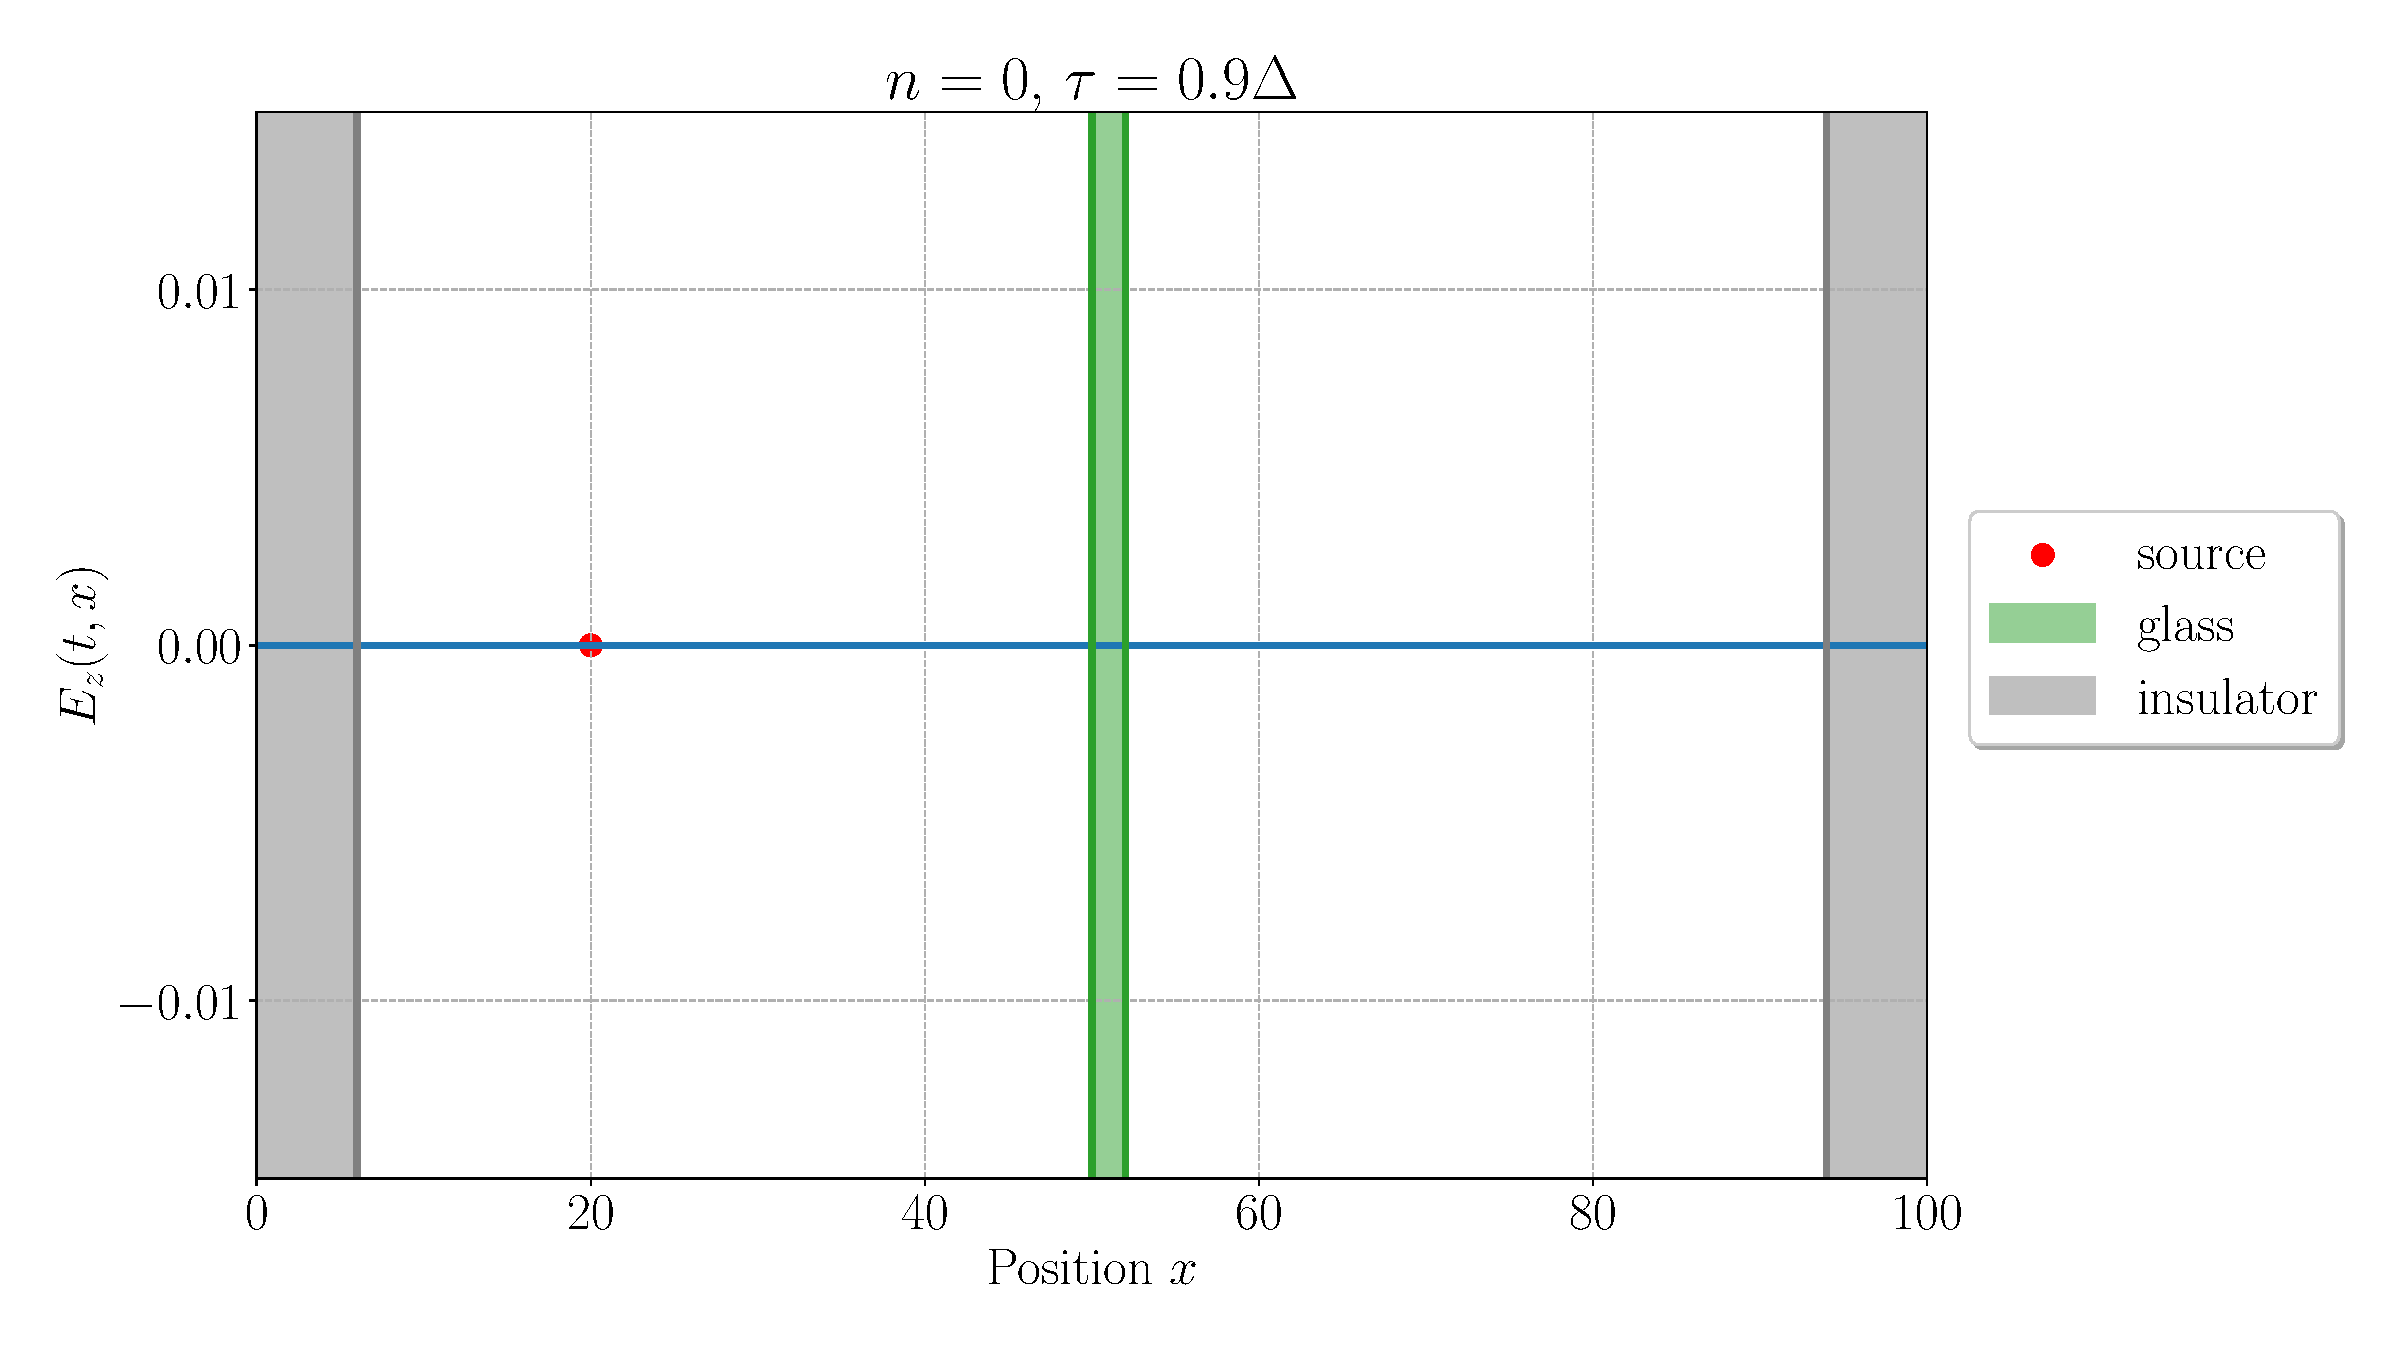
\includegraphics[width=0.9\textwidth]{Plots/maxwell_tau0.9_thinglass_nmax0.pdf}
         \caption{sketch of the overall system. The glass plate is depicted in green in the middle, and  at the system's boundaries there are two insulators (grey). The source at $x_s$ is represented by the red point.}
         \label{fig: sketch}
\end{figure}

A wave packet is generated by a source at $x_s$ (red dot), modeled as

\begin{equation}
    J_{source,z}(x,t) = \begin{cases}
        \sin(\omega t) e ^{-((t-30)/10)^2} & \text{if } x = x_s\\
        0 & \text{otherwise}
    \end{cases}.
    \label{eq: current}
\end{equation}

We impose boundary conditions $E_z(0,t) = E_z(X,t) = 0$, where $X$ is the domain length. The plate has permittivity $\epsilon$, permeability $\mu$, and refractive index $n_d$, while the surrounding medium is vacuum ($n=1$).

Assuming a linear, isotropic, nondispersive, and lossless medium with no free charges, Maxwell's equations reduce to:

\begin{align*}
\frac{\partial H_y}{\partial t} &= \frac{1}{\mu(x)}\left(\frac{\partial E_z}{\partial x} - \sigma^*(x) H_y\right)\\
\frac{\partial E_z}{\partial t} &= \frac{1}{\epsilon(x)}\left(\frac{\partial H_y}{\partial x} - J_{source,z}(x,t) - \sigma(x)E_z\right)
\end{align*}

We use the Yee algorithm with a staggered grid: $E_z$ at $x = l\Delta$ ($L+1$ points), $H_y$ at $x = (l+1/2)\Delta$ ($L$ points). Update equations:

\begin{align}
\begin{split}
H_y \Big|^{n+1}_{l+1/2} &= A_{l+1/2} H_y \Big|^{n}_{l+1/2} + B_{l+1/2} \frac{E_z \Big|^{n+1/2}_{l+1} - E_z \Big|^{n+1/2}_l}{\Delta} \\
E_z\Big|^{n+1/2}_l &= C_l E_z\Big|^{n-1/2}_l + D_l \left[\frac{H_y\Big|^n_{l+1/2} - H_y\Big|^n_{l-1/2}}{\Delta} - \delta_{l,i_s} J_{source}(n\tau)\right]
\end{split}
\label{eq: update_E_H}
\end{align}

with coefficients:

\begin{align*}
A_{l+1/2} &= \frac{1 - \frac{\sigma^* \tau}{2\mu}}{1 + \frac{\sigma^* \tau}{2\mu}}, &
B_{l+1/2} &= \frac{\frac{\tau}{\mu}}{1 + \frac{\sigma^* \tau}{2\mu}} \\
C_l &= \frac{1 - \frac{\sigma \tau}{2\epsilon}}{1 + \frac{\sigma \tau}{2\epsilon}}, &
D_l &= \frac{\frac{\tau}{\epsilon}}{1 + \frac{\sigma \tau}{2\epsilon}}
\end{align*}

The implementation in code:

\begin{align*}
    &\texttt{E[1:-1]} = {\texttt{D}_\texttt{l} \texttt{[1:-1]*(H[1:]-H[:-1])} \over \Delta} + \texttt{C}_\texttt{l}\texttt{[1:-1]*E[1:-1]}\\
    \\
    &\texttt{E[i}_\texttt{s}\texttt{]}\quad {-= }  \texttt{D}_\texttt{l}\texttt{[i}_\texttt{s}\texttt{]}\texttt{*}\texttt{J}_\texttt{source}\texttt{(n,}\tau\texttt{)}\\
    \\
    & \texttt{H} \qquad \quad = {\texttt{B}_\texttt{l}\texttt{[:-1]*(E[1:]-E[:-1])} \over \Delta} + \texttt{A}_\texttt{l}\texttt{[:-1]*H}.
\end{align*}

Only current and previous steps are stored to minimize memory use.

\subsection*{Reflection Coefficient}
The reflection coefficient is defined as:

\begin{equation}
R := \frac{|E^\text{max}_\text{reflected}|^2}{|E^\text{max}_\text{incident}|^2}
\label{eq: R}
\end{equation}

We identify maxima in the intervals $t_{\text{in}} = [1700\tau, 2000\tau]$ and $t_{\text{ref}} = [4700\tau, 4950\tau]$ using \texttt{np.max}, focusing on spatial indices $l \geq 1000$ to avoid transmitted components.

\clearpage
\section{Results}
In this section, we present the results for two different systems.
\subsection{The Thin Glass Plate}
The first system was already discussed in the previous section and \refFig{fig: sketch}, containing two insulators at the boundaries and a thin glass plate in the center. Mathematically, the insulators are described by the electrical conductivity $\sigma$ and the magnetic loss $\sigma^*$

\begin{equation}
    \sigma (x) = \sigma^* (x) = 
    \begin{cases}
        1 \quad \text{if} \quad 0 \leq x \leq 6 \lambda \\
        0 \quad \text{if} \quad 6 \lambda < x < L \Delta - 6 \lambda \\
        1 \quad \text{if} \quad L \Delta - 6 \lambda \leq x \leq L \Delta.
    \end{cases}
    \label{eq: sigma}
\end{equation}

\noindent Further, the glass plate is described by the electric permittivity
\begin{equation}
    \epsilon (x)=
    \begin{cases}
        1   \quad &\text{if} \quad 0 \leq x < L \Delta/2 \\
        n_d^2 \quad &\text{if} \quad L \Delta/2 \leq x < L \Delta/2 + 2 \lambda \\
        1   \quad &\text{if} \quad L \Delta/2 + 2 \lambda \leq x \leq L \Delta,
    \end{cases}
\end{equation}
where $n_d$ is the refractive index of the glass with $n_d=1.46$.\footnote{In the code, both, the $\sigma$ and $\epsilon$ can simply be implemented via \texttt{if}-statements} Moreover, the system has a constant magnetic permeability
\begin{equation}
    \mu(x) = 1.
\end{equation}

In \refFig{fig: Maxwell_thin}, the results for the different times (a) $n=2500$ $(t\approx 45)$, (b) $n=3500$ $(t\approx 63)$, (c) $n=3510$ $(t\approx 63)$, (d) $n=4500$ $(t\approx 81)$, and (e) $n=20000$ $(t\approx360)$, and $\tau=1.05 \Delta=0.021$ for (f) $n=500$ $(t\approx 9)$ are presented and the parameters of the system are $\lambda=1$, $\Delta=\lambda/50=0.02$, $\tau=0.9 \Delta=0.018$, $X=L\Delta=100 \lambda=100$, and $L=5000$.

\begin{figure}[h!]
     \begin{subfigure}[h]{0.499\textwidth}
         \centering
         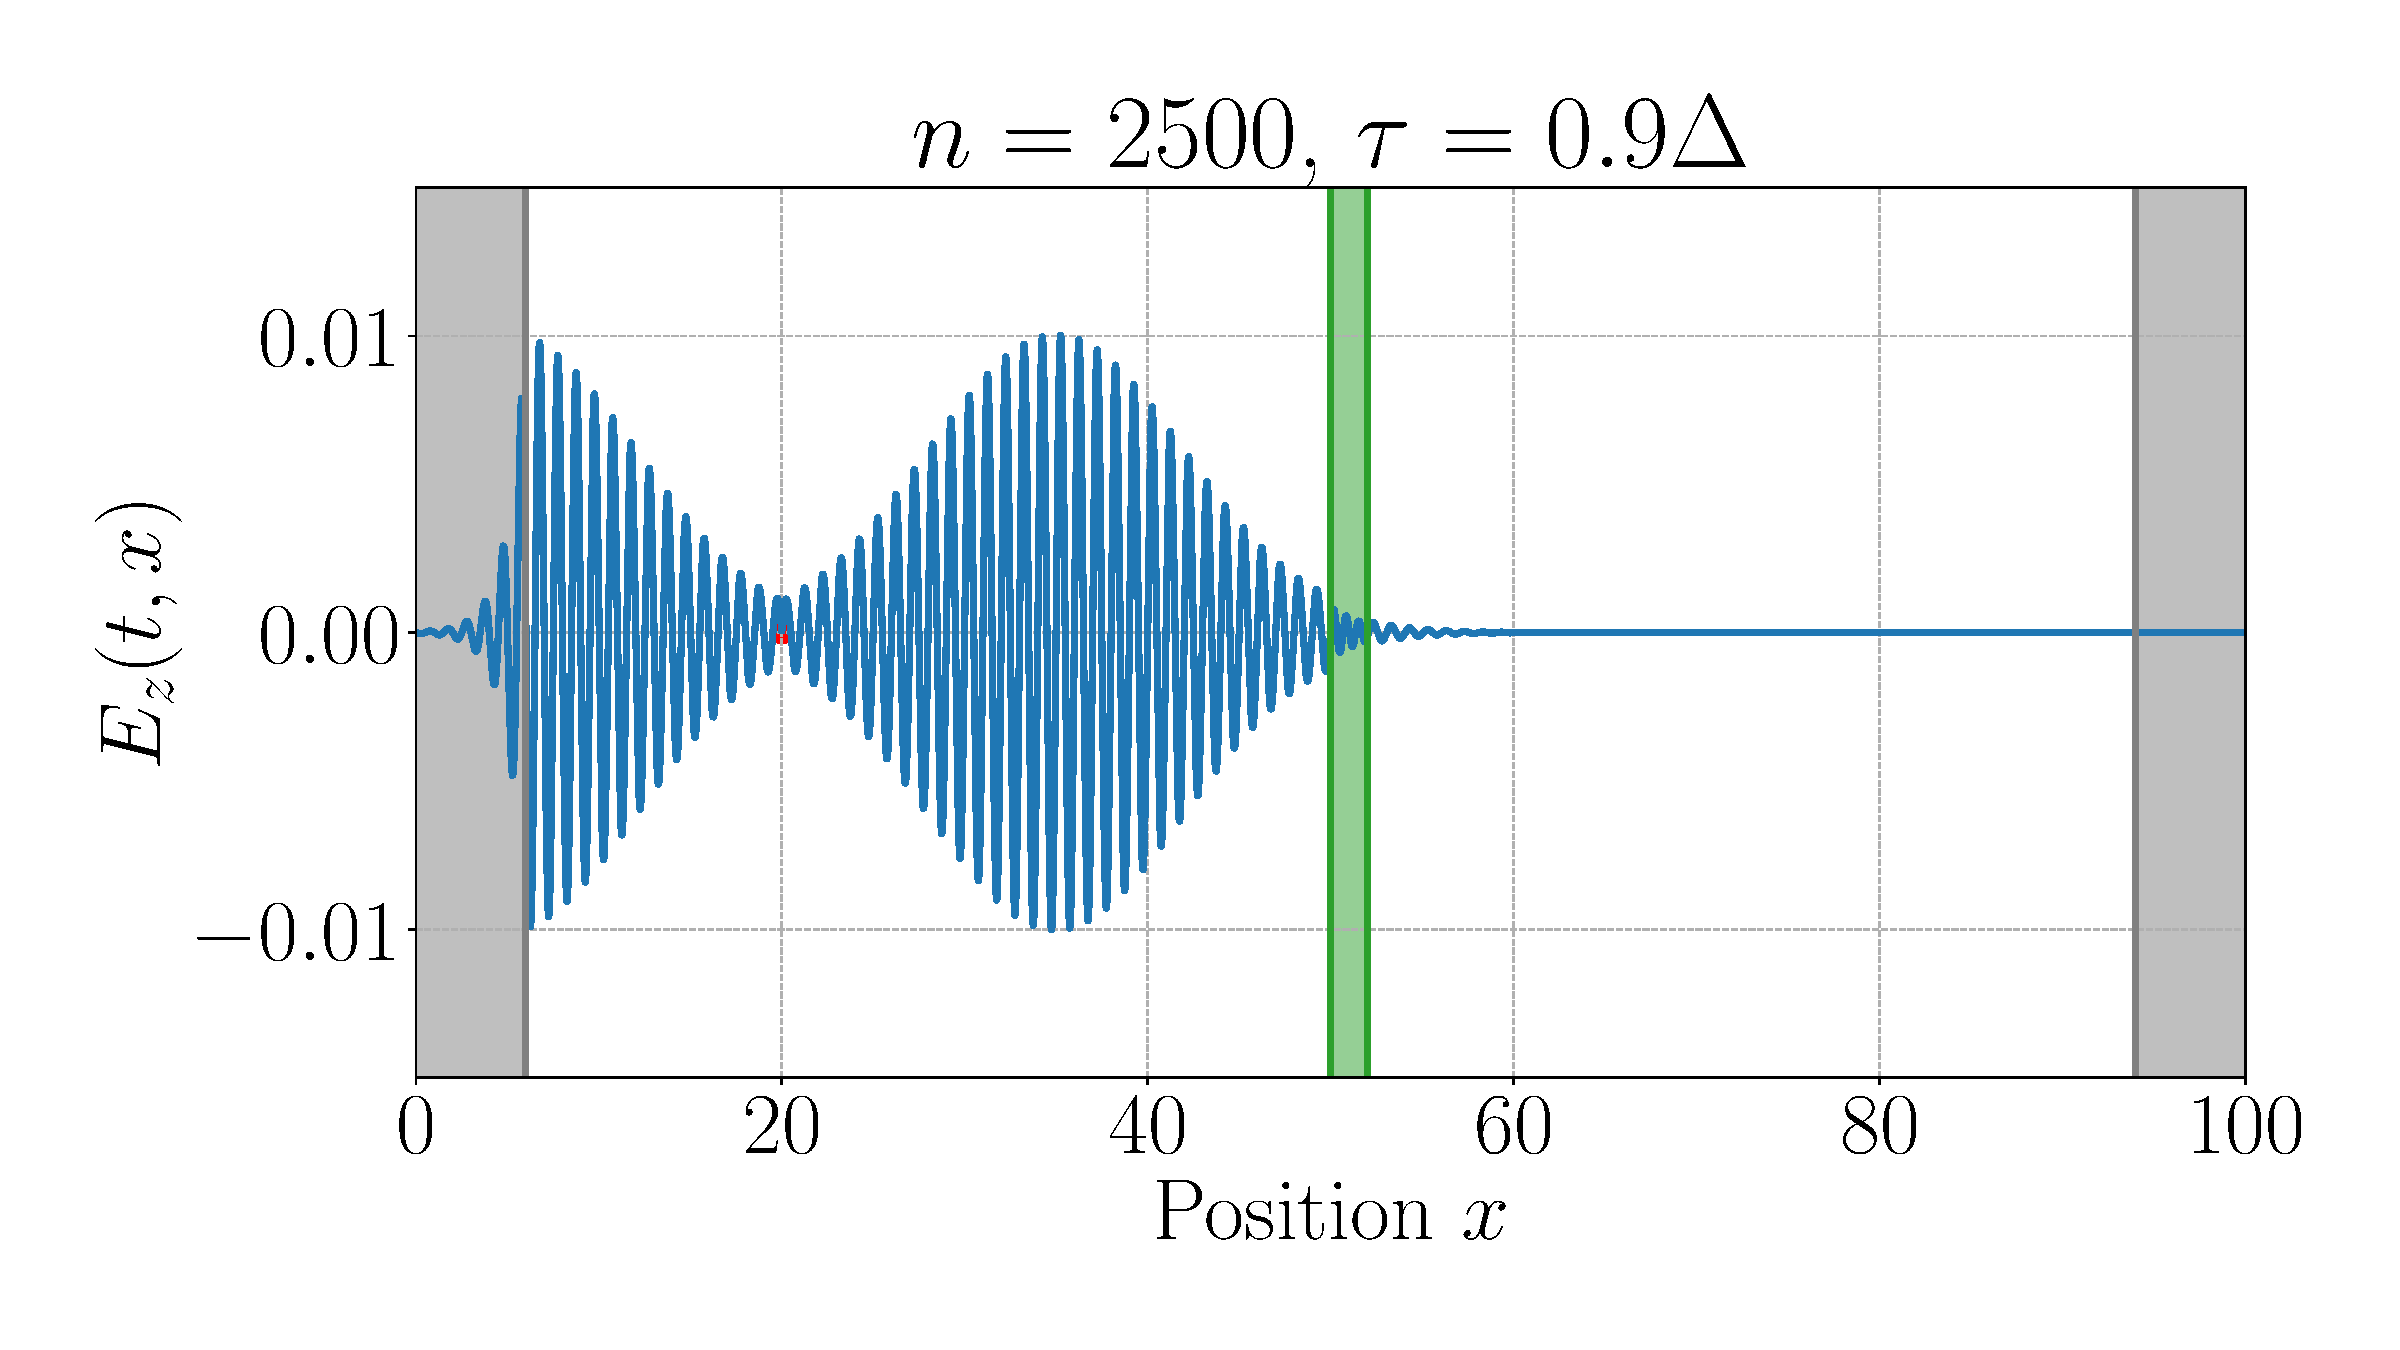
\includegraphics[width=\textwidth]{Plots/maxwell_tau0.9_thinglass_nmax2500.pdf}
         \caption{}
         \label{fig: thin_t40_tau09}
     \end{subfigure}
     \begin{subfigure}[h]{0.499\textwidth}
         \centering
         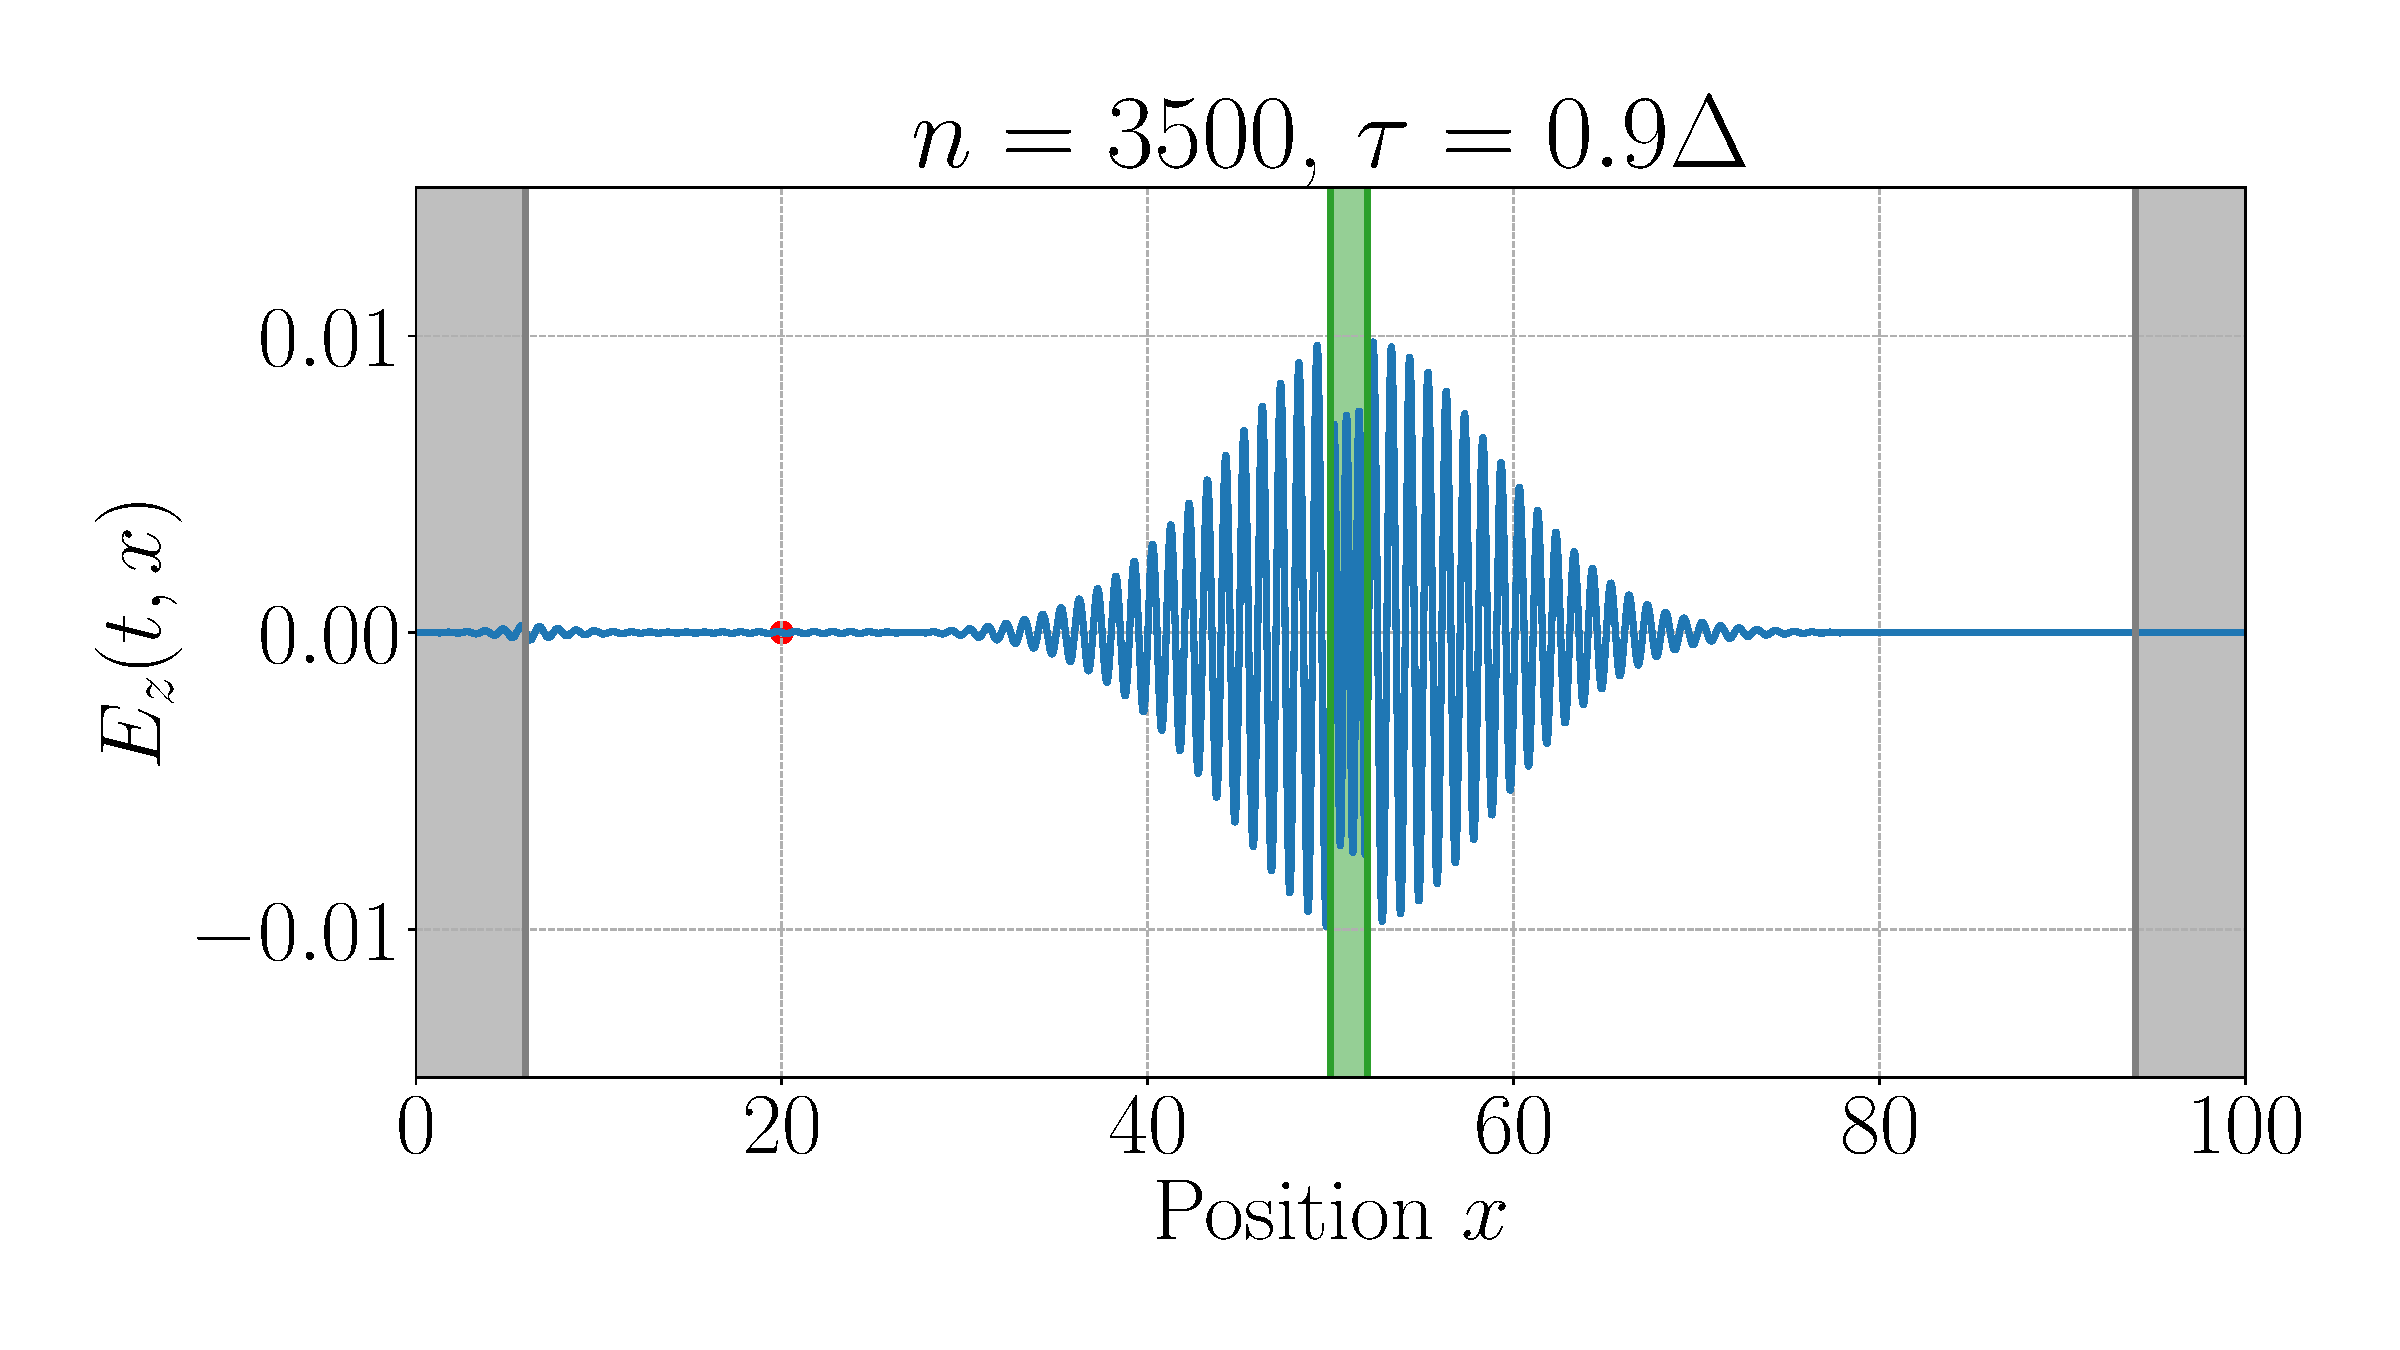
\includegraphics[width=\textwidth]{Plots/maxwell_tau0.9_thinglass_nmax3500.pdf}
         \caption{}
         \label{fig: thin_t60_tau09}
     \end{subfigure}
     \begin{subfigure}[h]{0.499\textwidth}
         \centering
         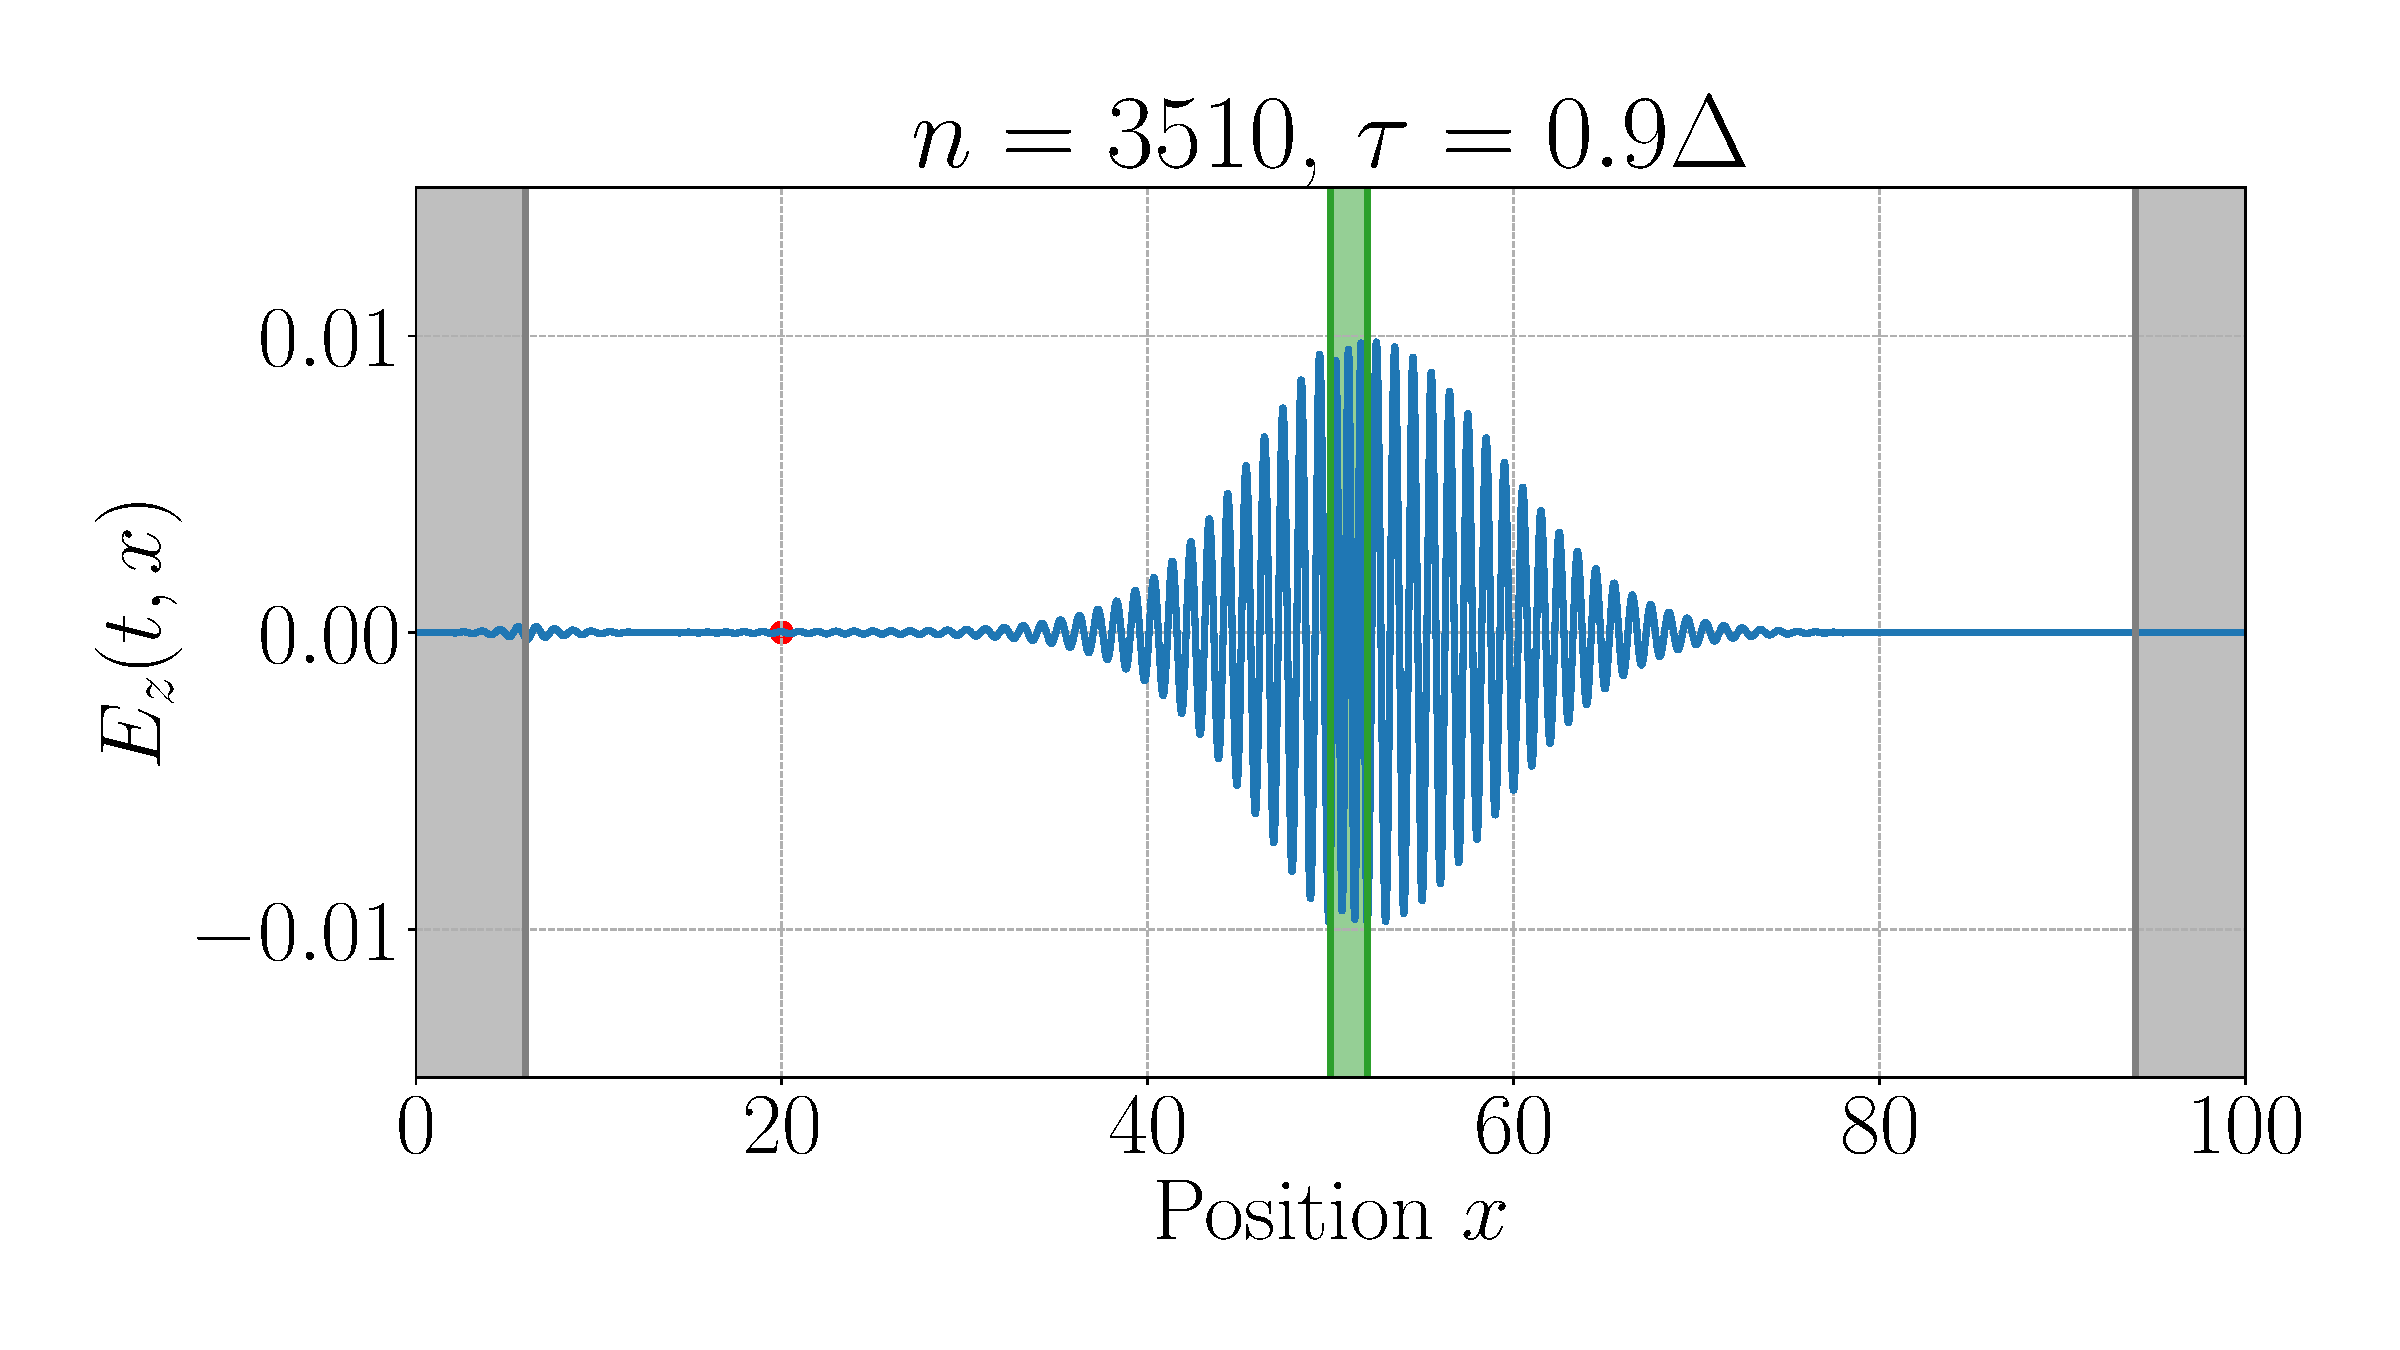
\includegraphics[width=\textwidth]{Plots/maxwell_tau0.9_thinglass_nmax3510.pdf}
         \caption{}
         \label{fig: thin_n3505_tau09}
     \end{subfigure}
     \begin{subfigure}[h]{0.499\textwidth}
         \centering
         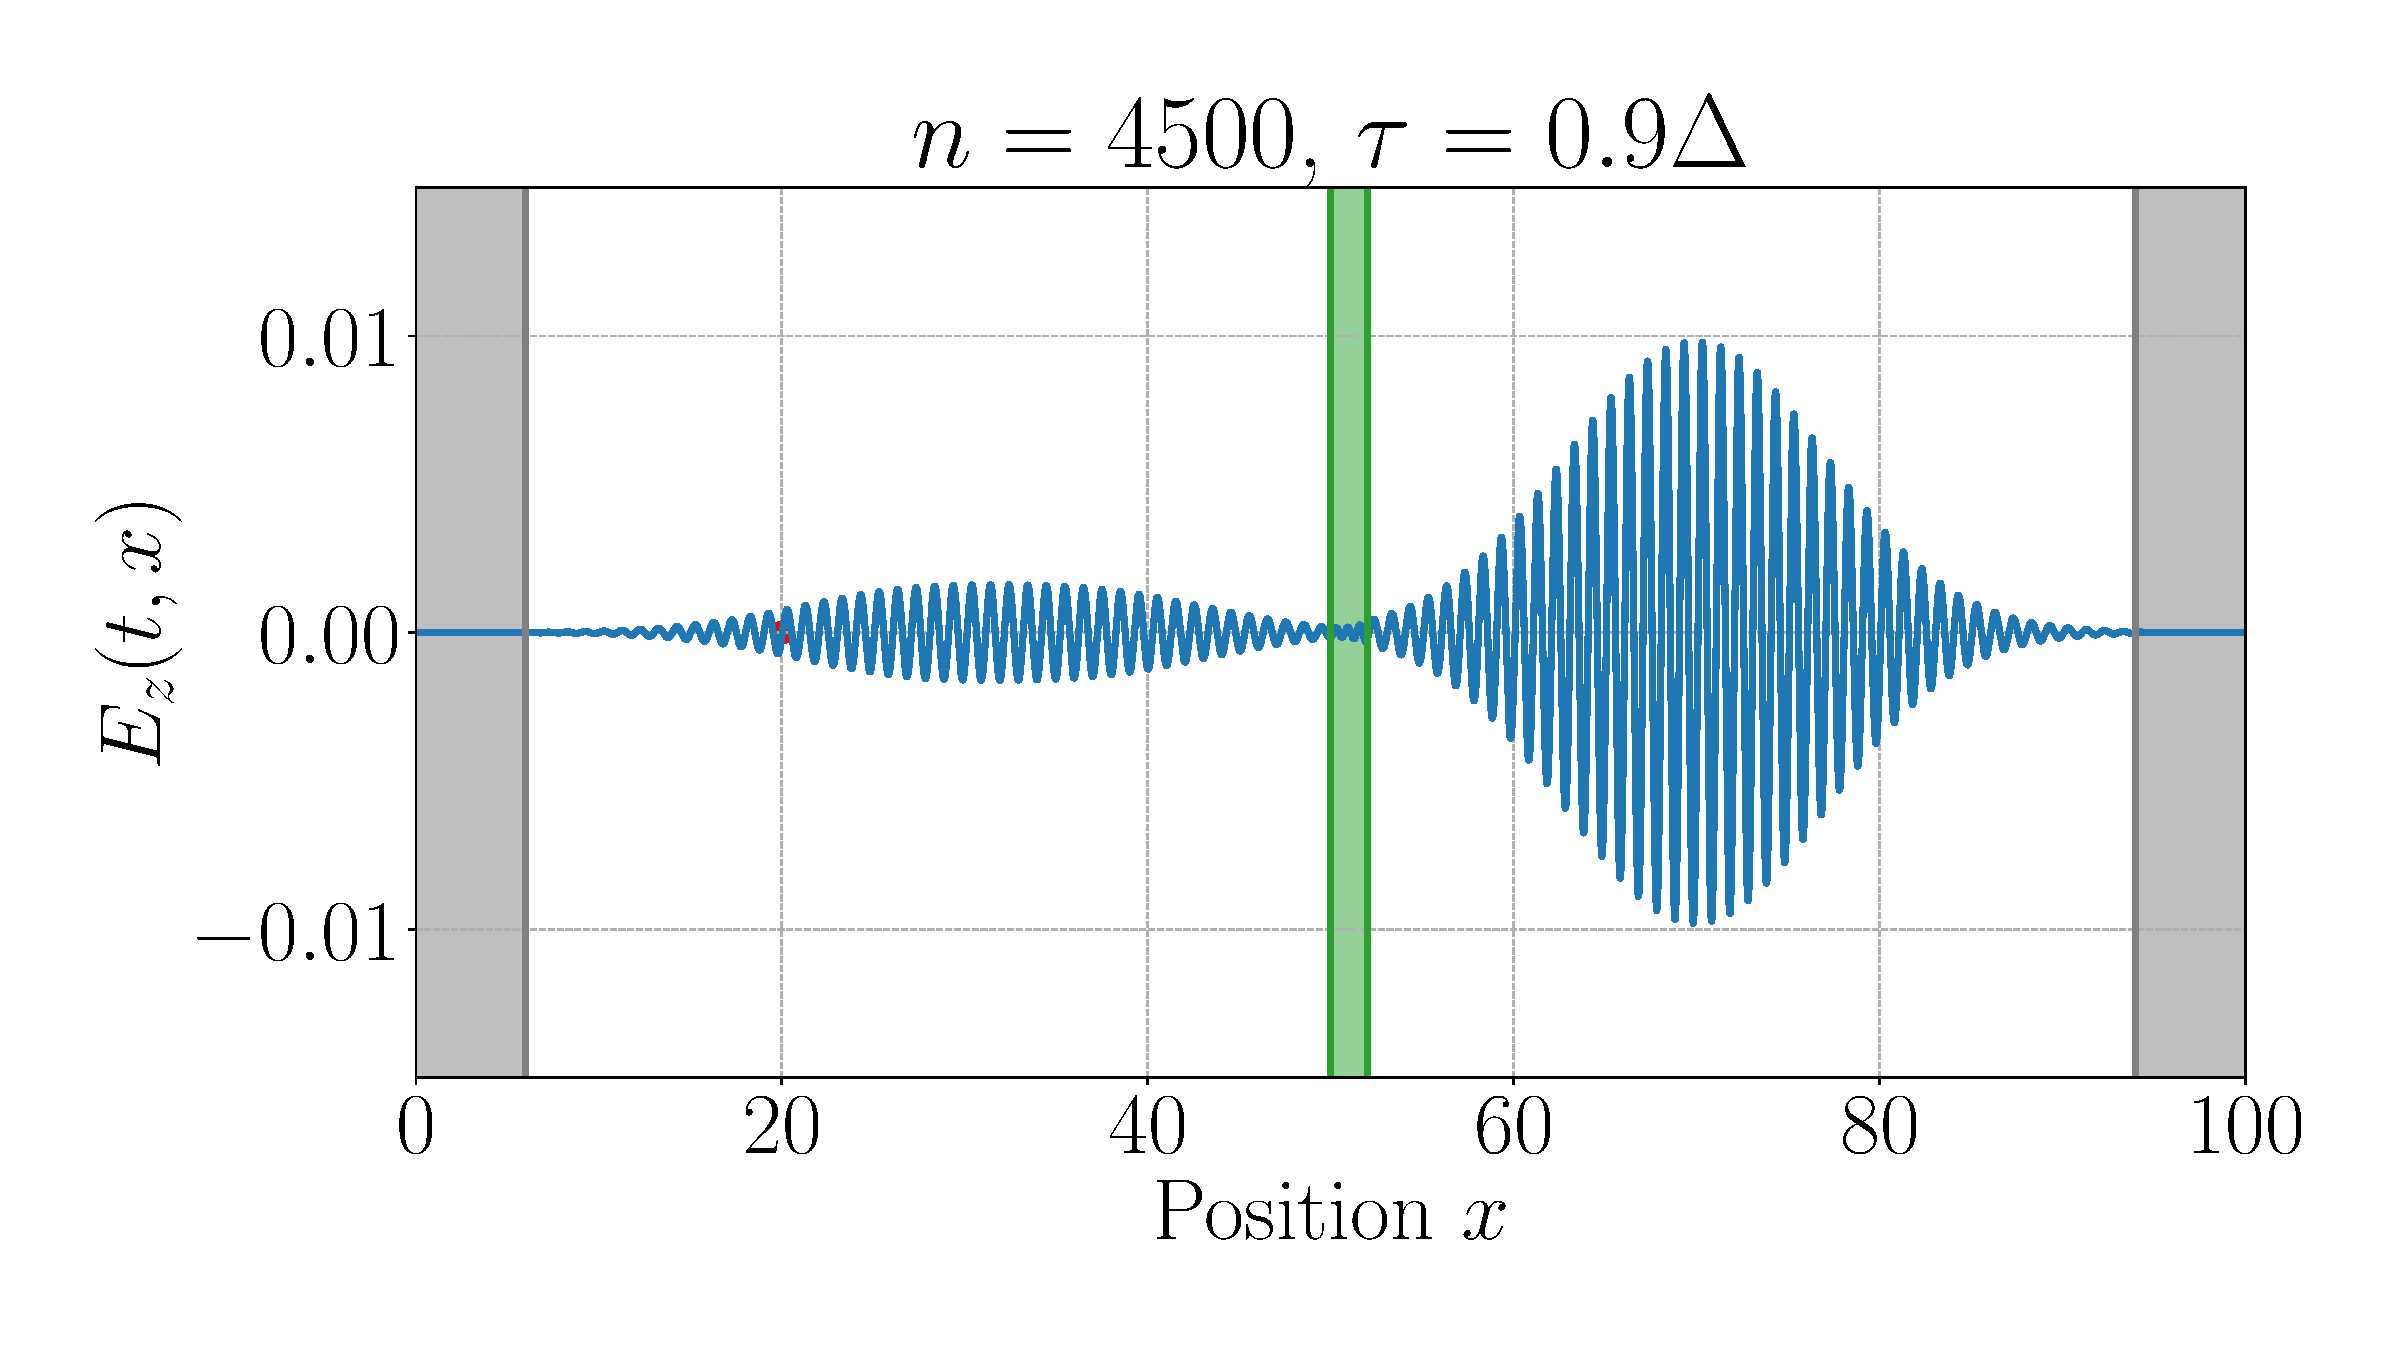
\includegraphics[width=\textwidth]{Plots/maxwell_tau0.9_thinglass_nmax4500.pdf}
         \caption{}
         \label{fig: thin_t80_tau09}
     \end{subfigure}
     \begin{subfigure}[h]{0.499\textwidth}
         \centering
         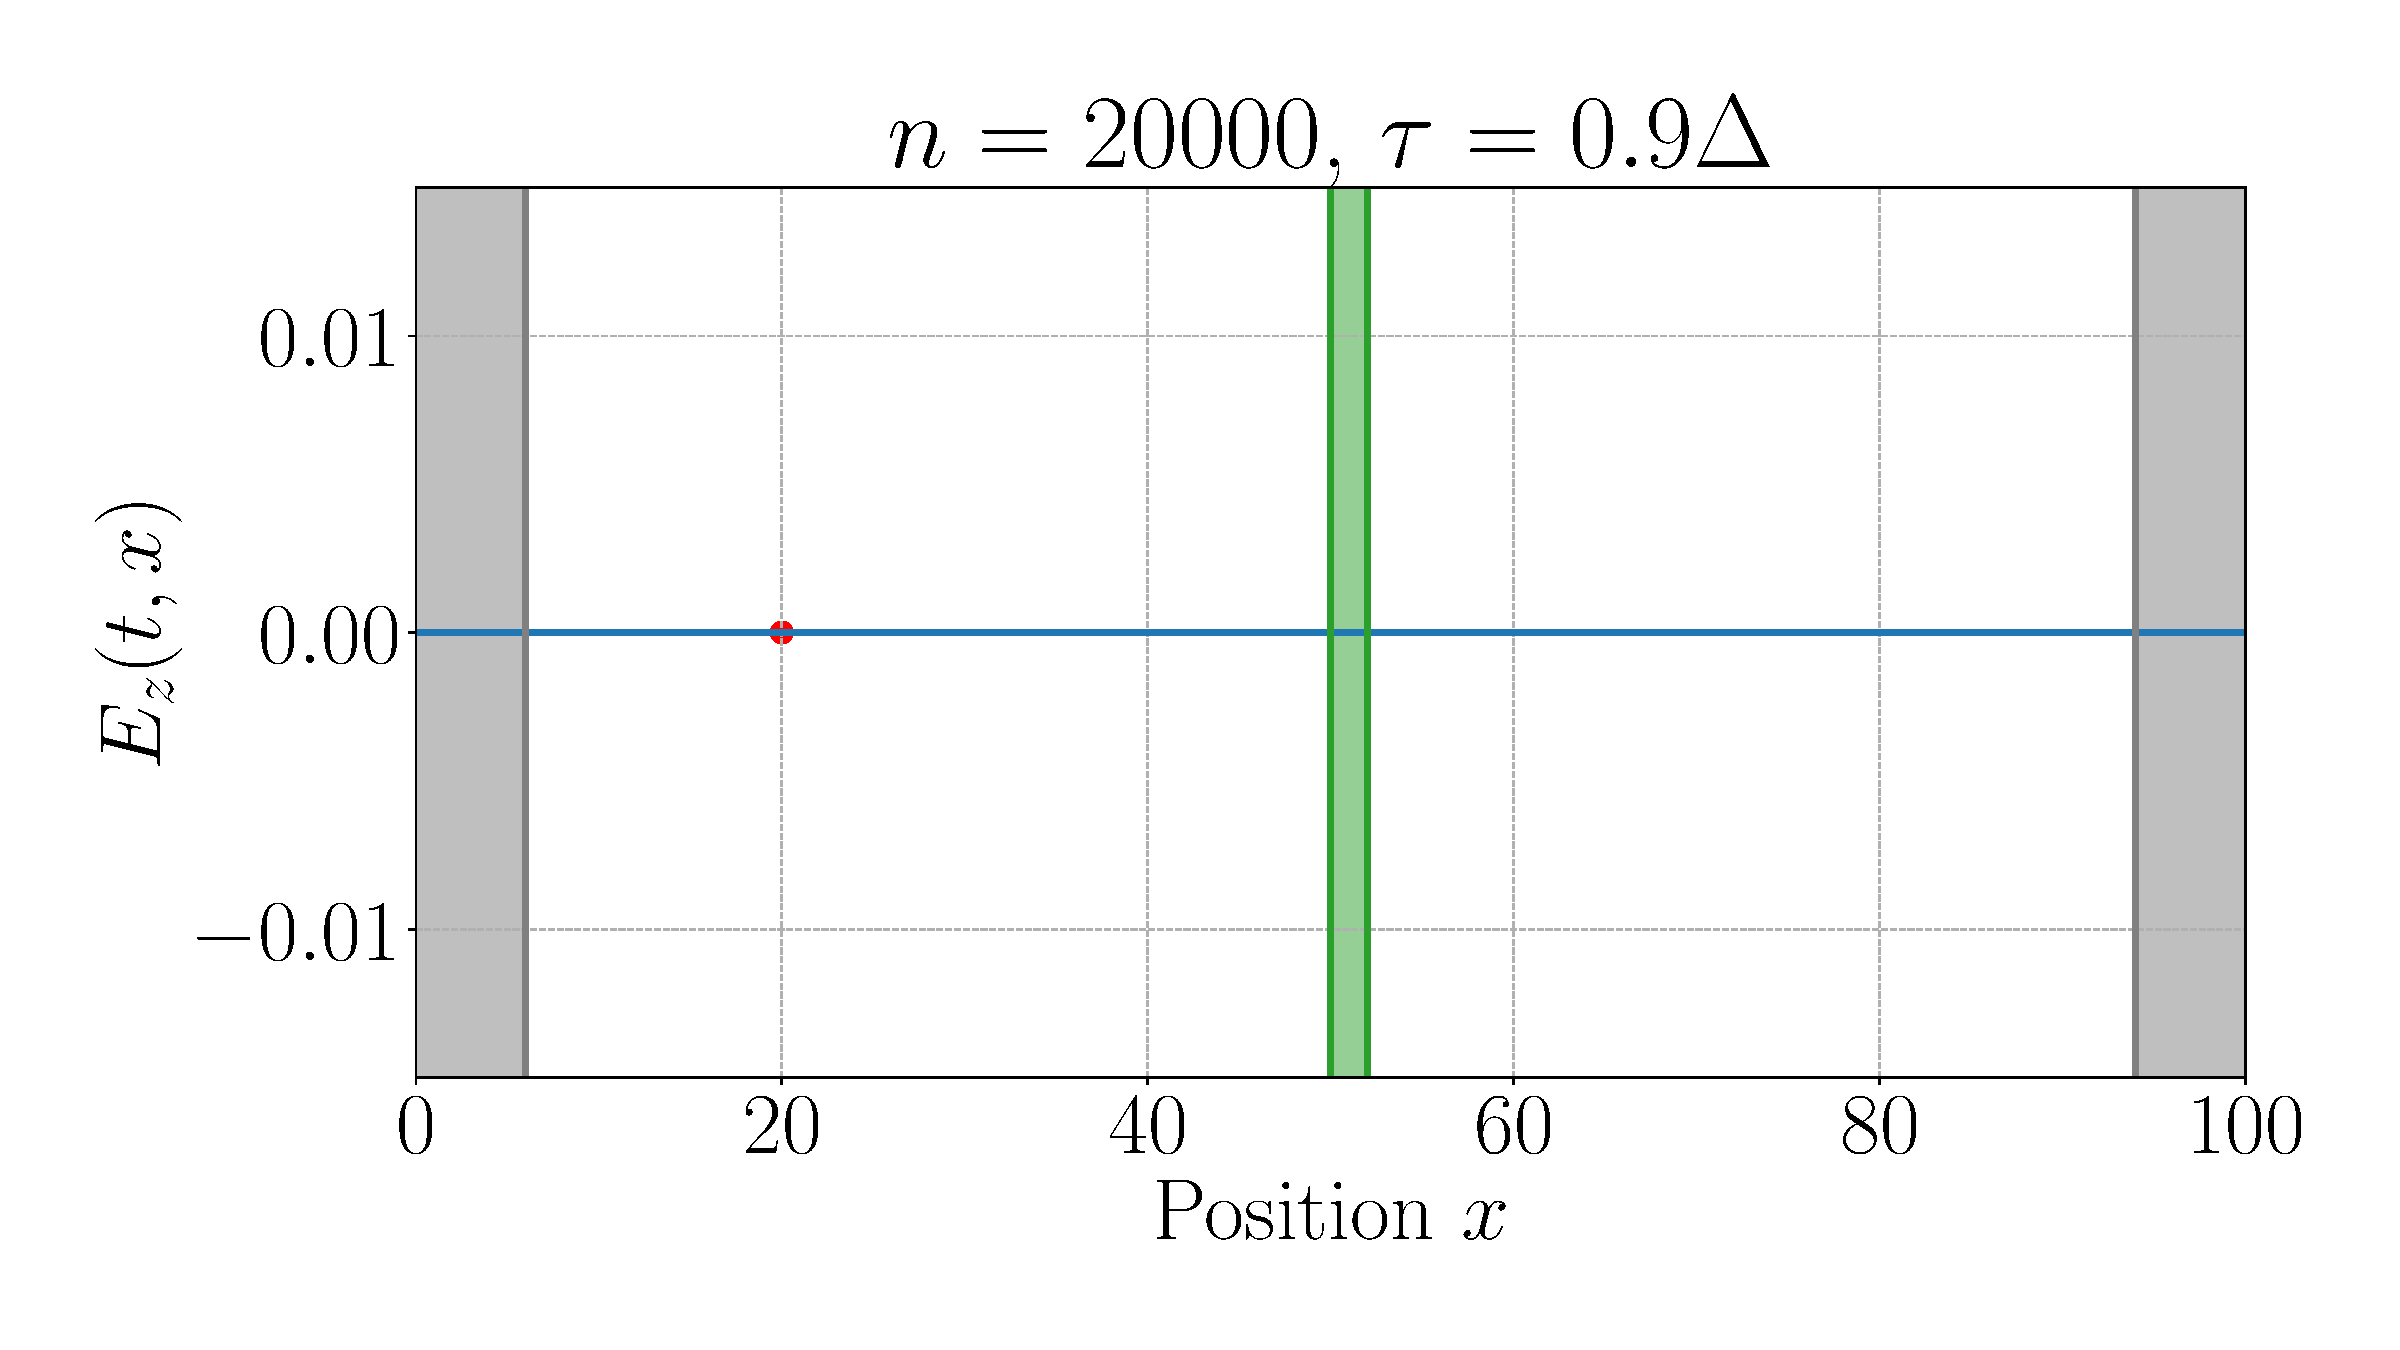
\includegraphics[width=\textwidth]{Plots/maxwell_tau0.9_thinglass_nmax20000.pdf}
         \caption{}
         \label{fig: thin_t500_tau09}
     \end{subfigure}
     \begin{subfigure}[h]{0.499\textwidth}
         \centering
         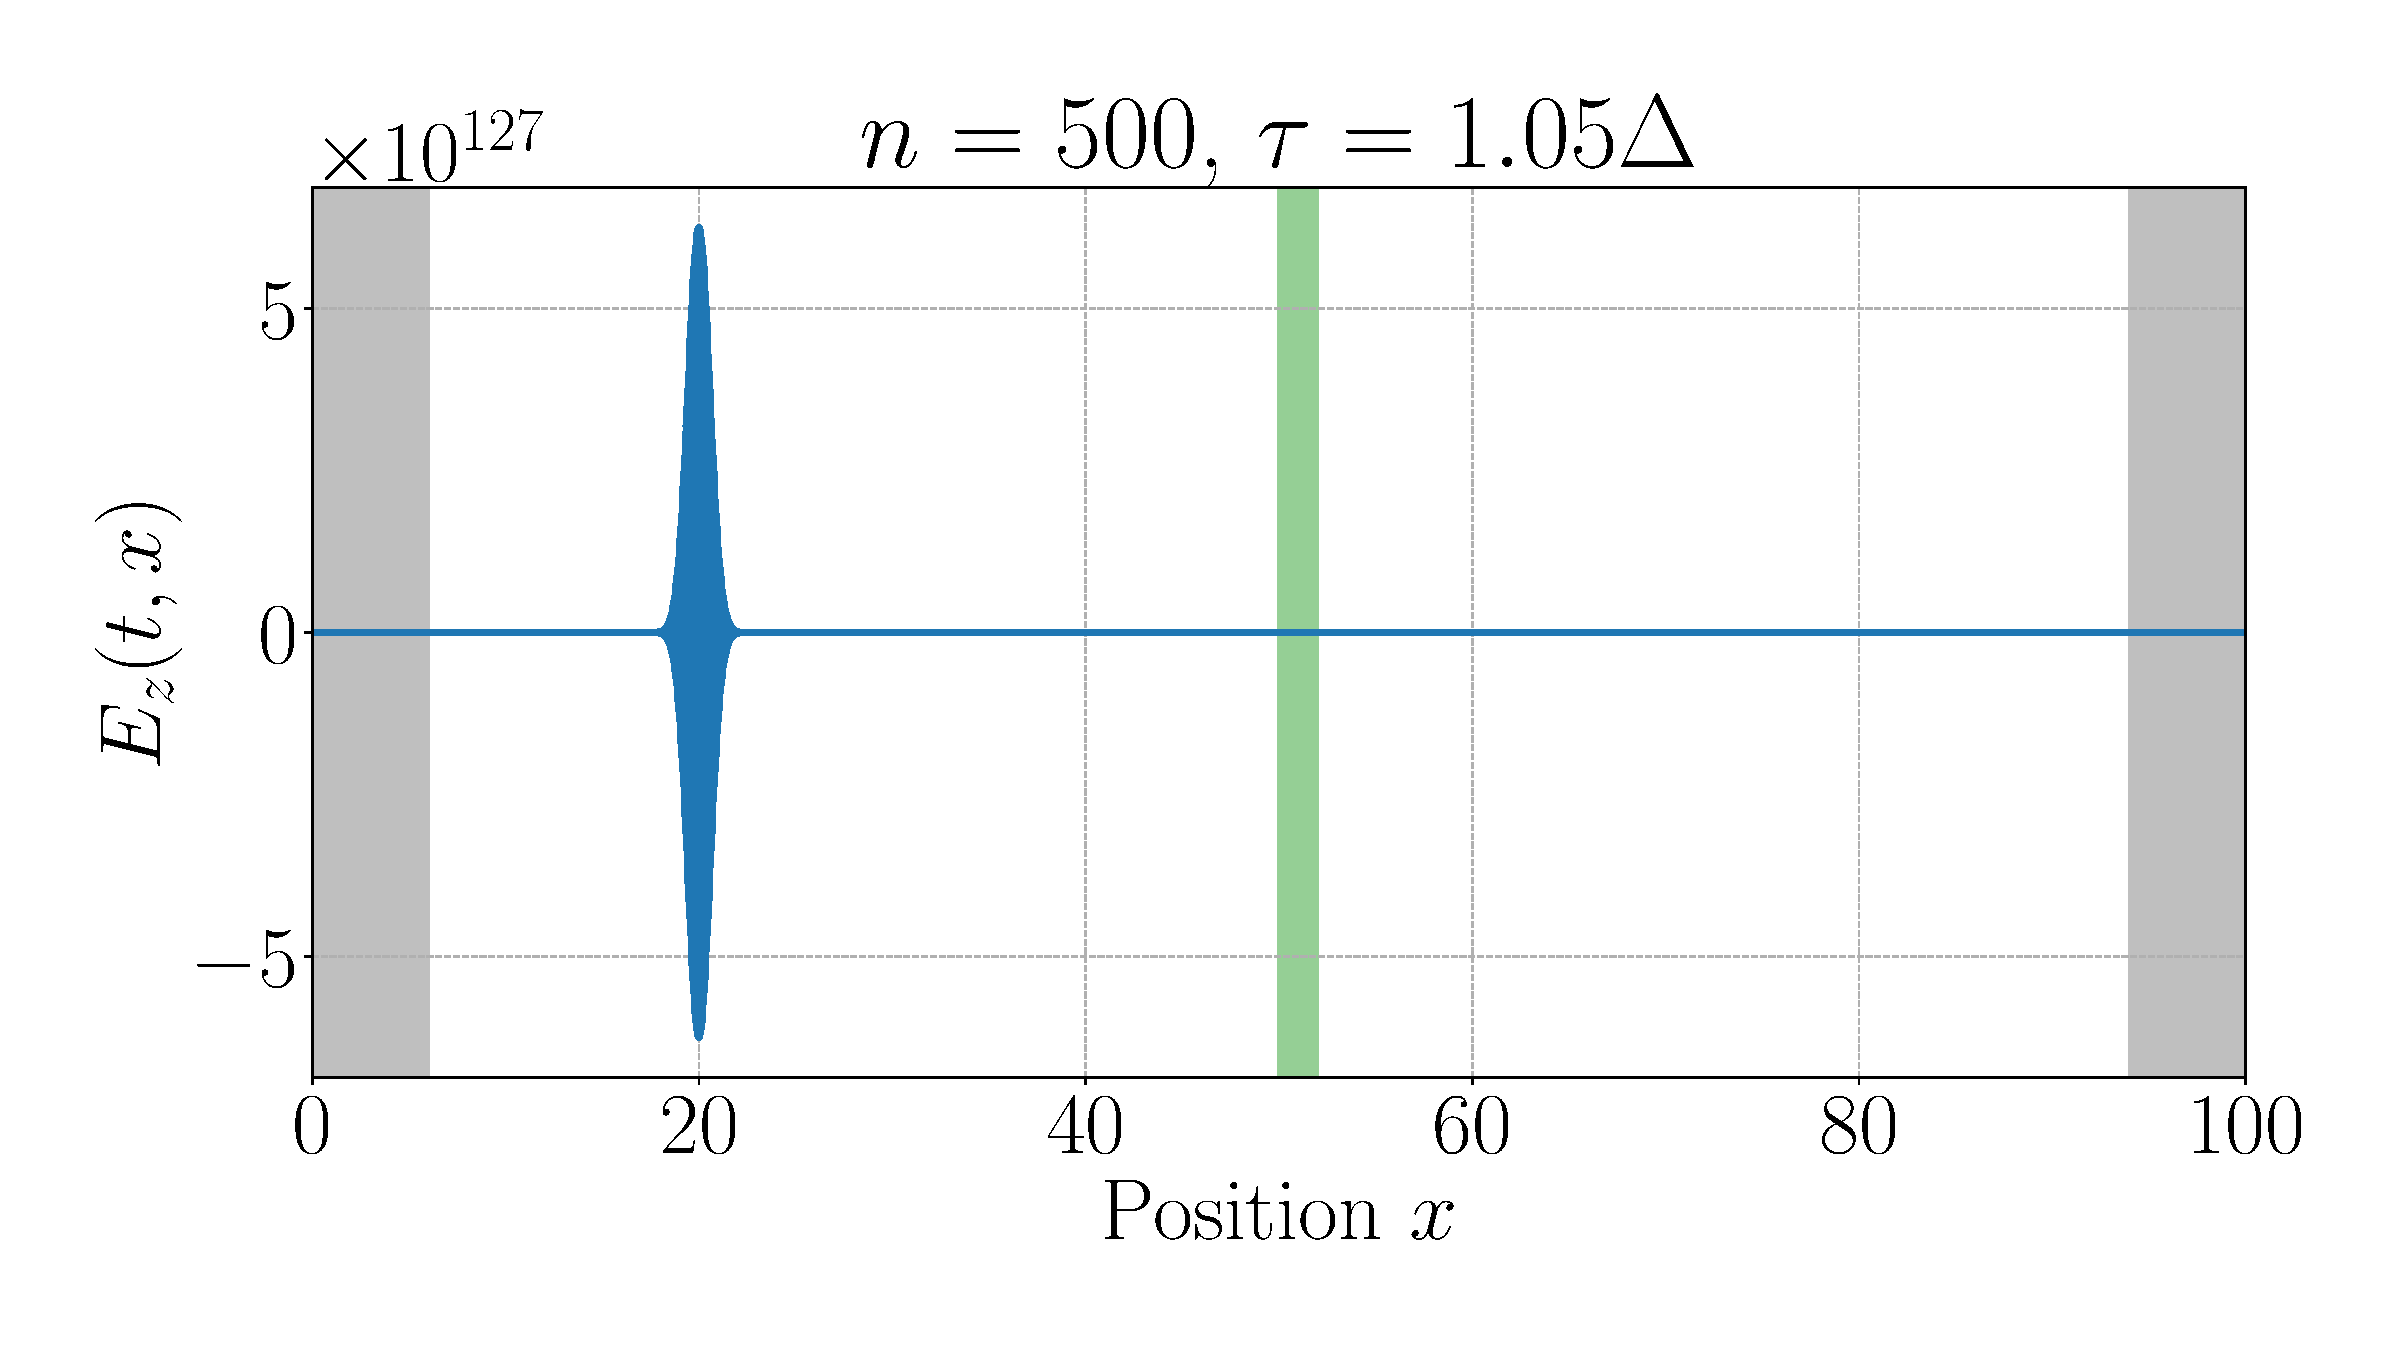
\includegraphics[width=\textwidth]{Plots/maxwell_tau1.05_thinglass_nmax500.pdf}
         \caption{}
         \label{fig: thin_t10_tau105}
     \end{subfigure}
\caption{Numerical solutions of the Maxwell equations using the Yee algorithm in one dimension for the system with the thin glass plate. The figures show the z-component of the electric field. The plots contain the glass plate in green and the insulator insulators in grey. The discretizations are $\lambda=1$, $\Delta=\lambda/50=0.02$, $\tau=0.9 \Delta=0.018$, $X=L\Delta=100 \lambda=100$, and $L=5000$. The plots show the solution of the algorithm at different times: (a) $n=2500$ $(t\approx 45)$, (b) $n=3500$ $(t\approx 63)$, (c) $n=3510$ $(t\approx 63)$, (d) $n=4500$ $(t\approx 81)$, and (e) $n=20000$ $(t\approx360)$, and $\tau=1.05 \Delta=0.021$ for (f) $n=500$ $(t\approx 9)$.}
\label{fig: Maxwell_thin}
\end{figure}
\clearpage

\subsection{The Thick Glass Plate}
The second system that we study is very similar. The electrical conductivity $\sigma$, the magnetic loss $\sigma^*$, and the magnetic permeability $\mu$ are the same as before. However, now, we consider a thick glass plate that extends from the middle up to the end of the simulated spatial interval. This is described by the electric permittivity\footnote{In the code, this can simply be implemented via \texttt{if}-statements}
\begin{equation}
    \epsilon (x)=
    \begin{cases}
        1       &\quad \text{if} \quad 0 \leq x < L \Delta/2 \\
        n_d^2   &\quad \text{if} \quad L \Delta/2 \leq x < L \Delta,
    \end{cases}
    \label{eq: eps thick}
\end{equation}
where we have the same refractive index $n_d=1.46$. This system, at its initial time $t=0$, can be seen in \refFig{fig: thick_t0_tau09}. The obtained simulation results are presented in \refFig{fig: Maxwell_thick} for the times $t$ and time discretisations $\tau$. \\

\begin{figure}[h!]
     \begin{subfigure}[h]{0.499\textwidth}
         \centering
         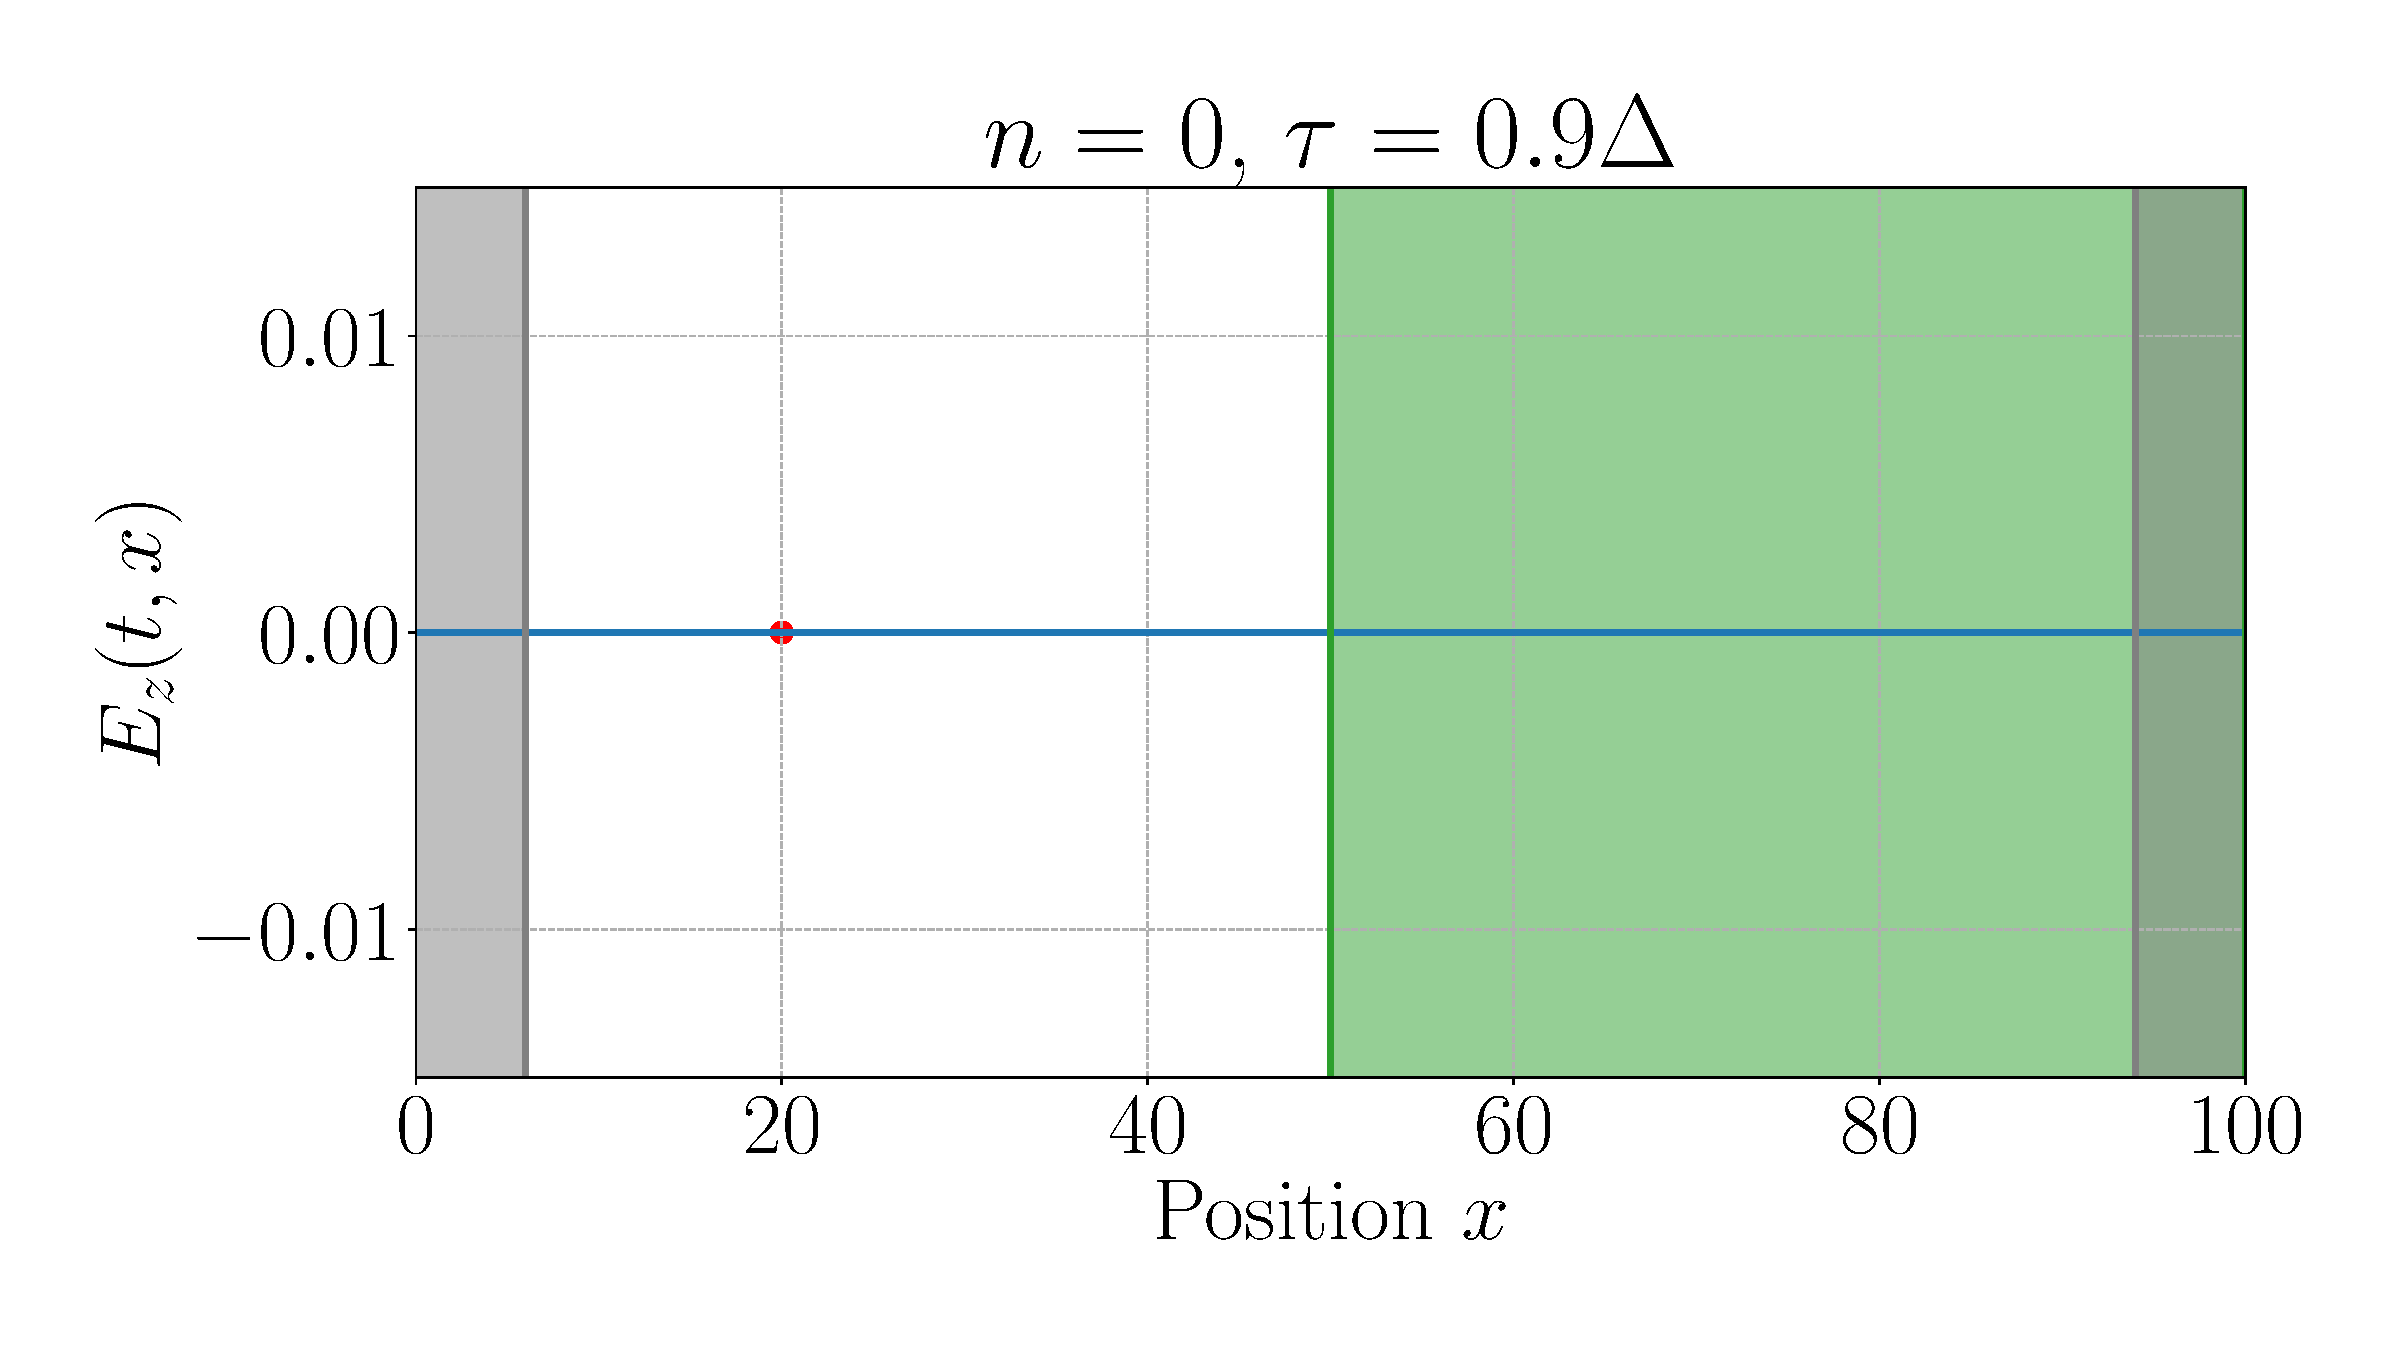
\includegraphics[width=\textwidth]{Plots/maxwell_tau0.9_thickglass_nmax0.pdf}
         \caption{}
         \label{fig: thick_t0_tau09}
     \end{subfigure}
     \begin{subfigure}[h]{0.499\textwidth}
         \centering
         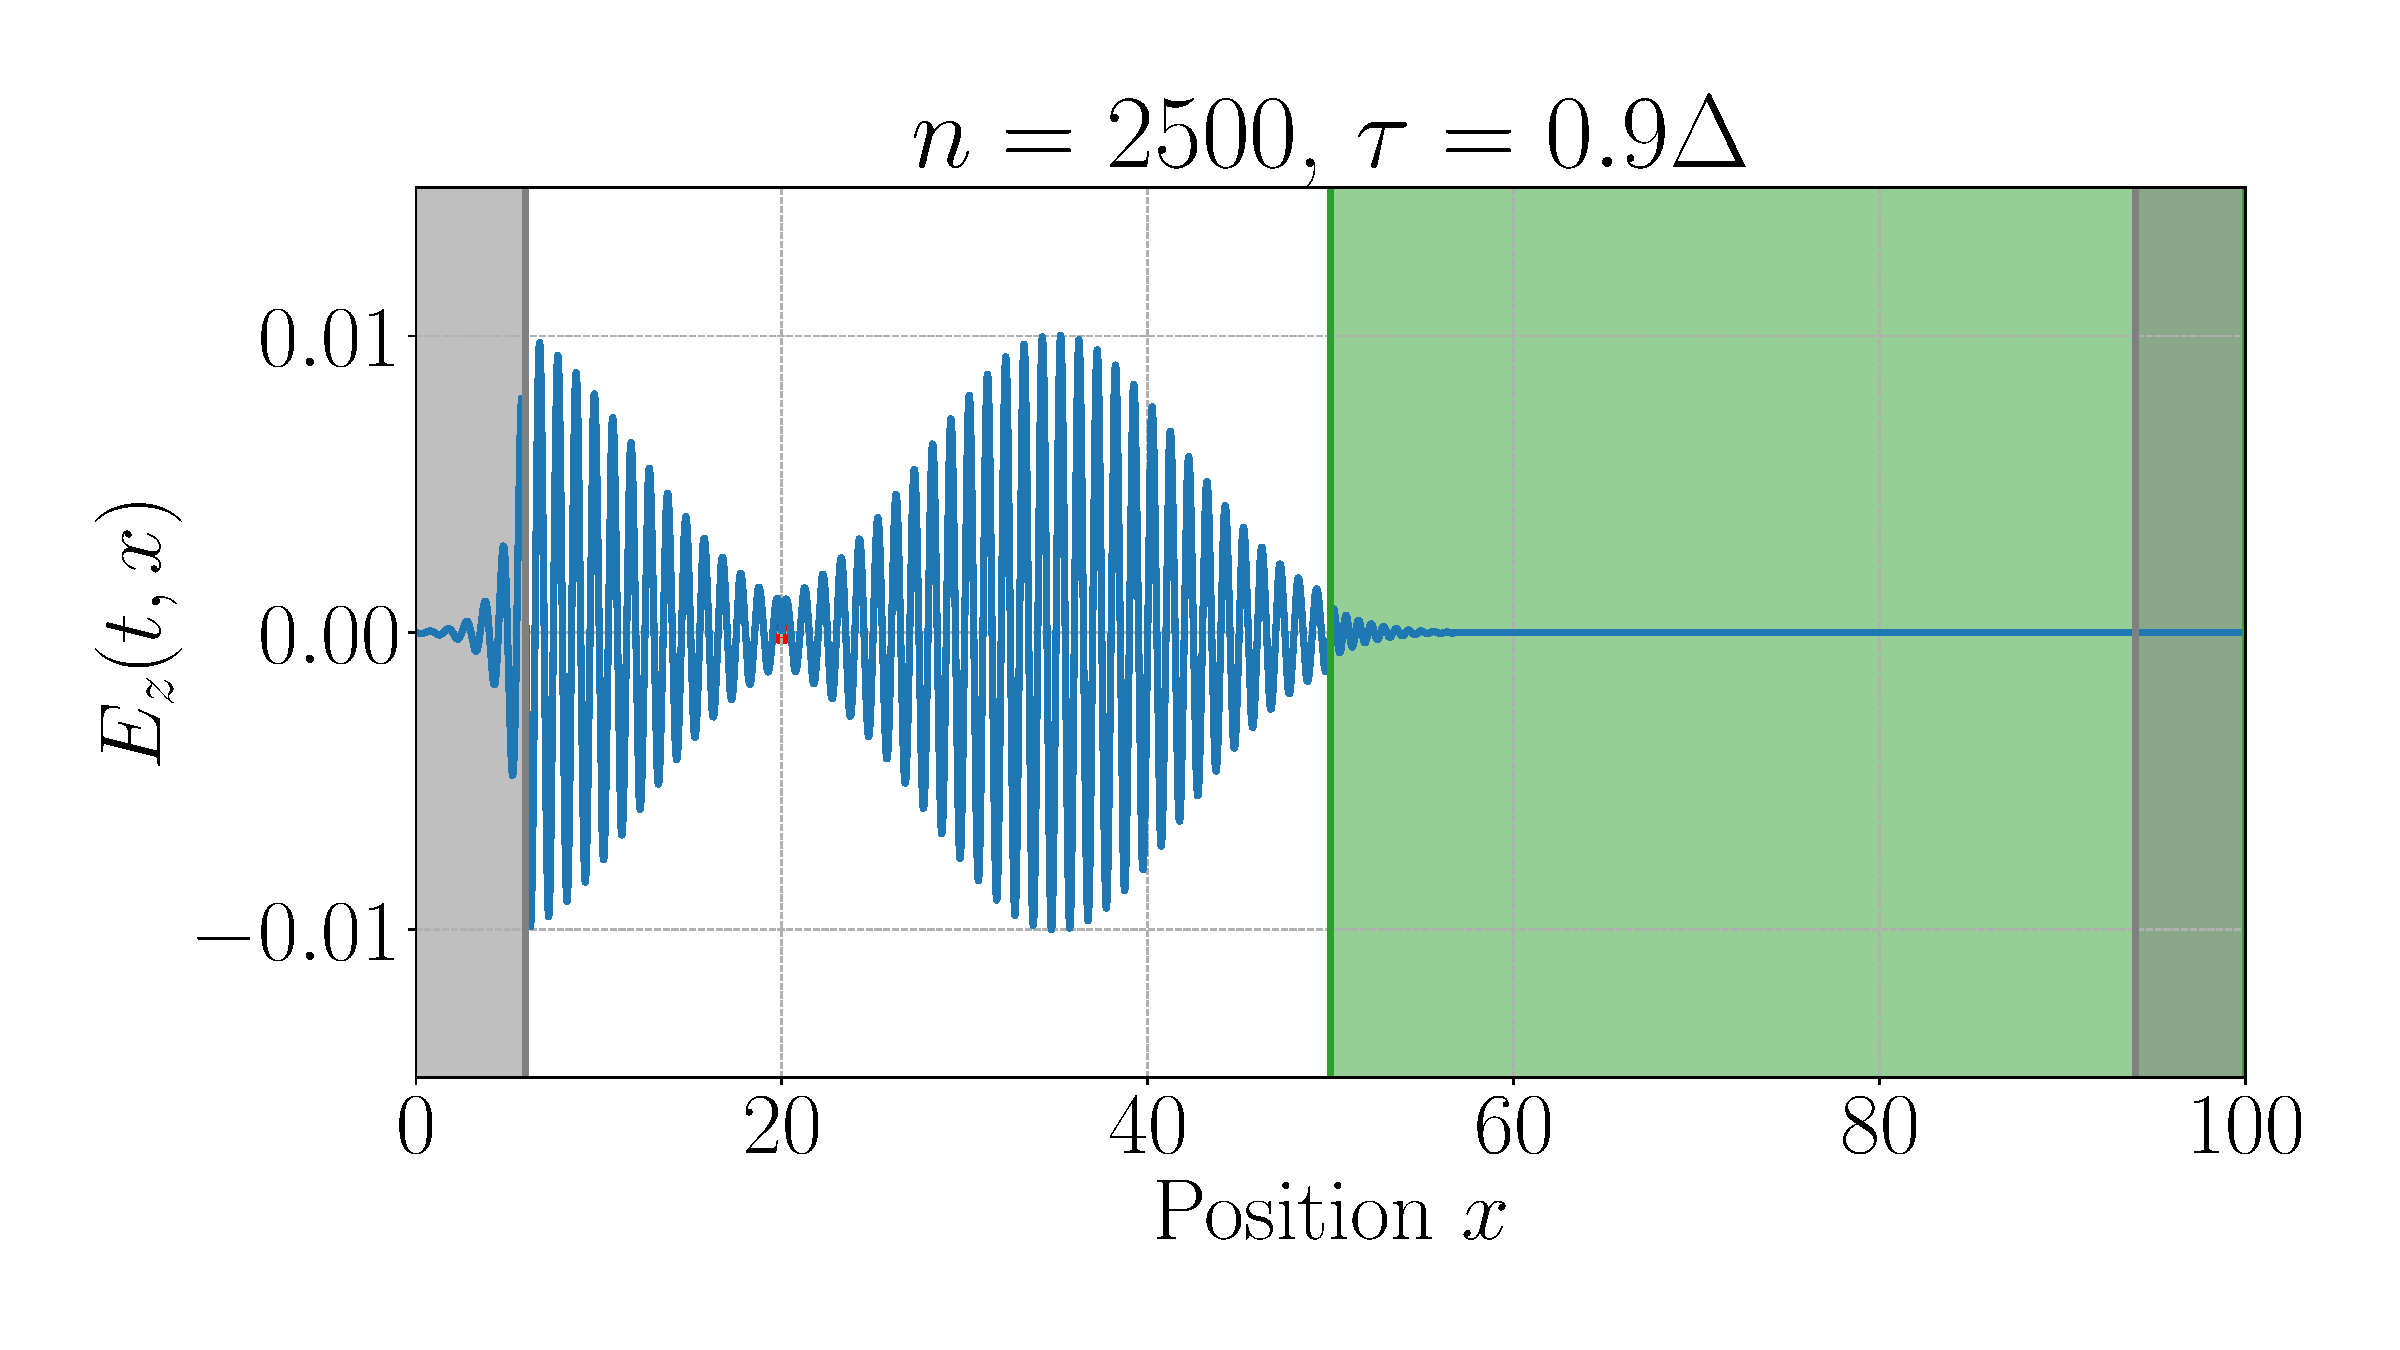
\includegraphics[width=\textwidth]{Plots/maxwell_tau0.9_thickglass_nmax2500.pdf}
         \caption{}
         \label{fig: thick_t40_tau09}
     \end{subfigure}
     \begin{subfigure}[h]{0.499\textwidth}
         \centering
         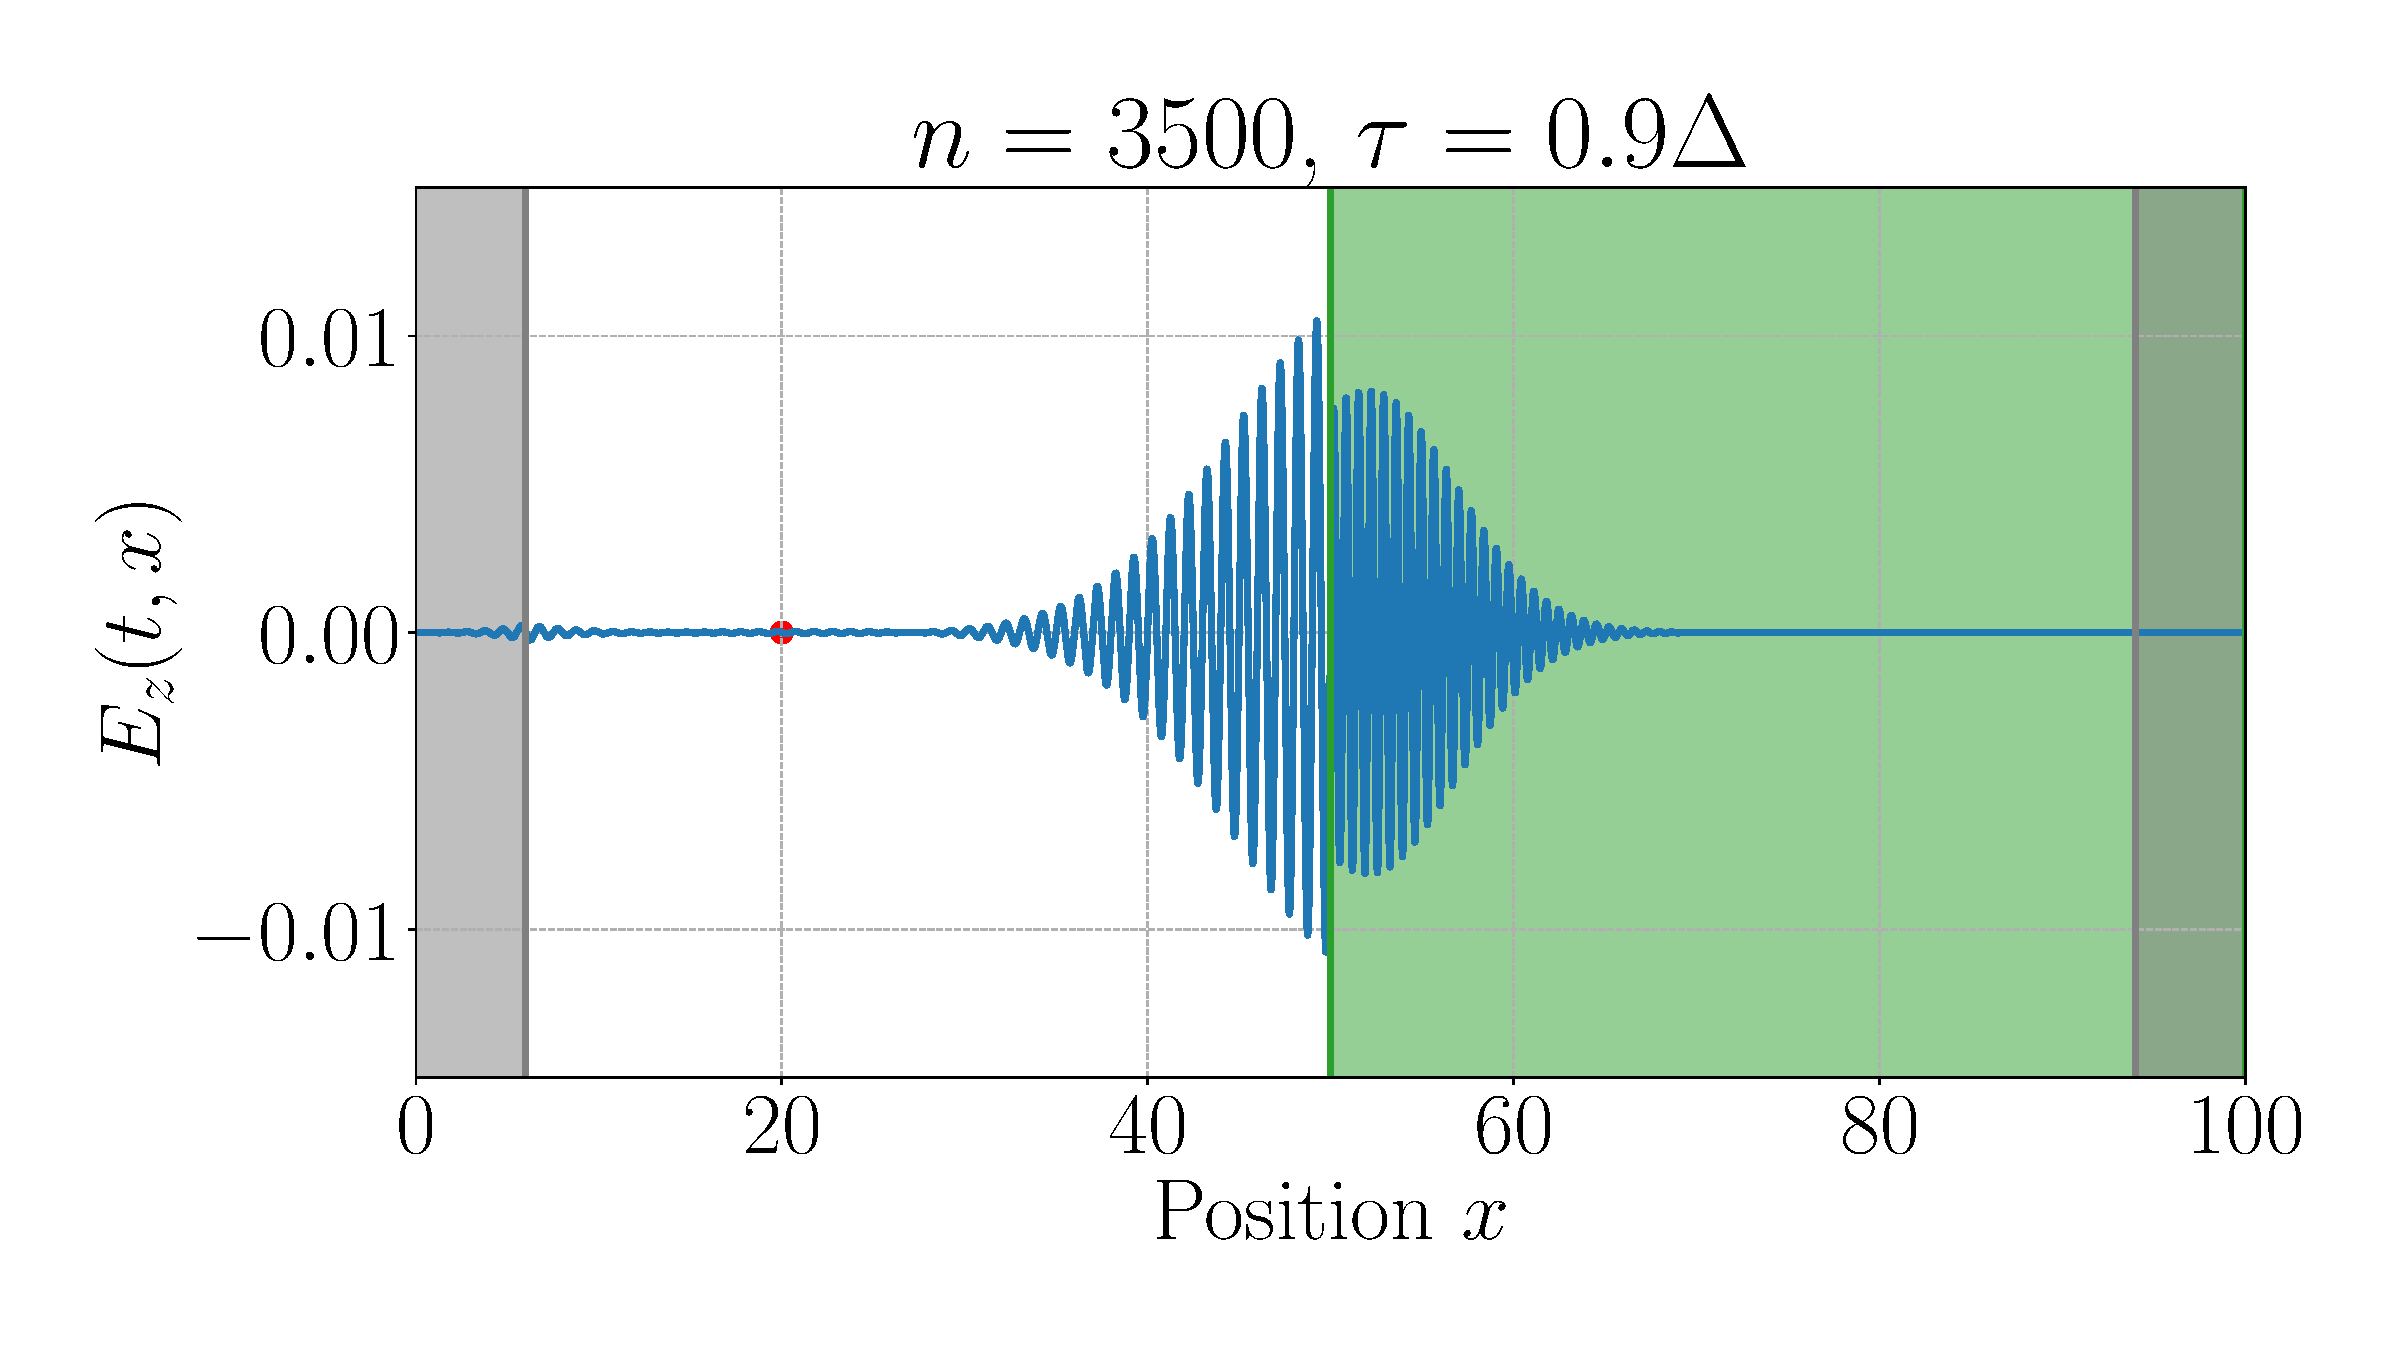
\includegraphics[width=\textwidth]{Plots/maxwell_tau0.9_thickglass_nmax3500.pdf}
         \caption{}
         \label{fig: thick_t60_tau09}
     \end{subfigure}
     \begin{subfigure}[h]{0.499\textwidth}
         \centering
         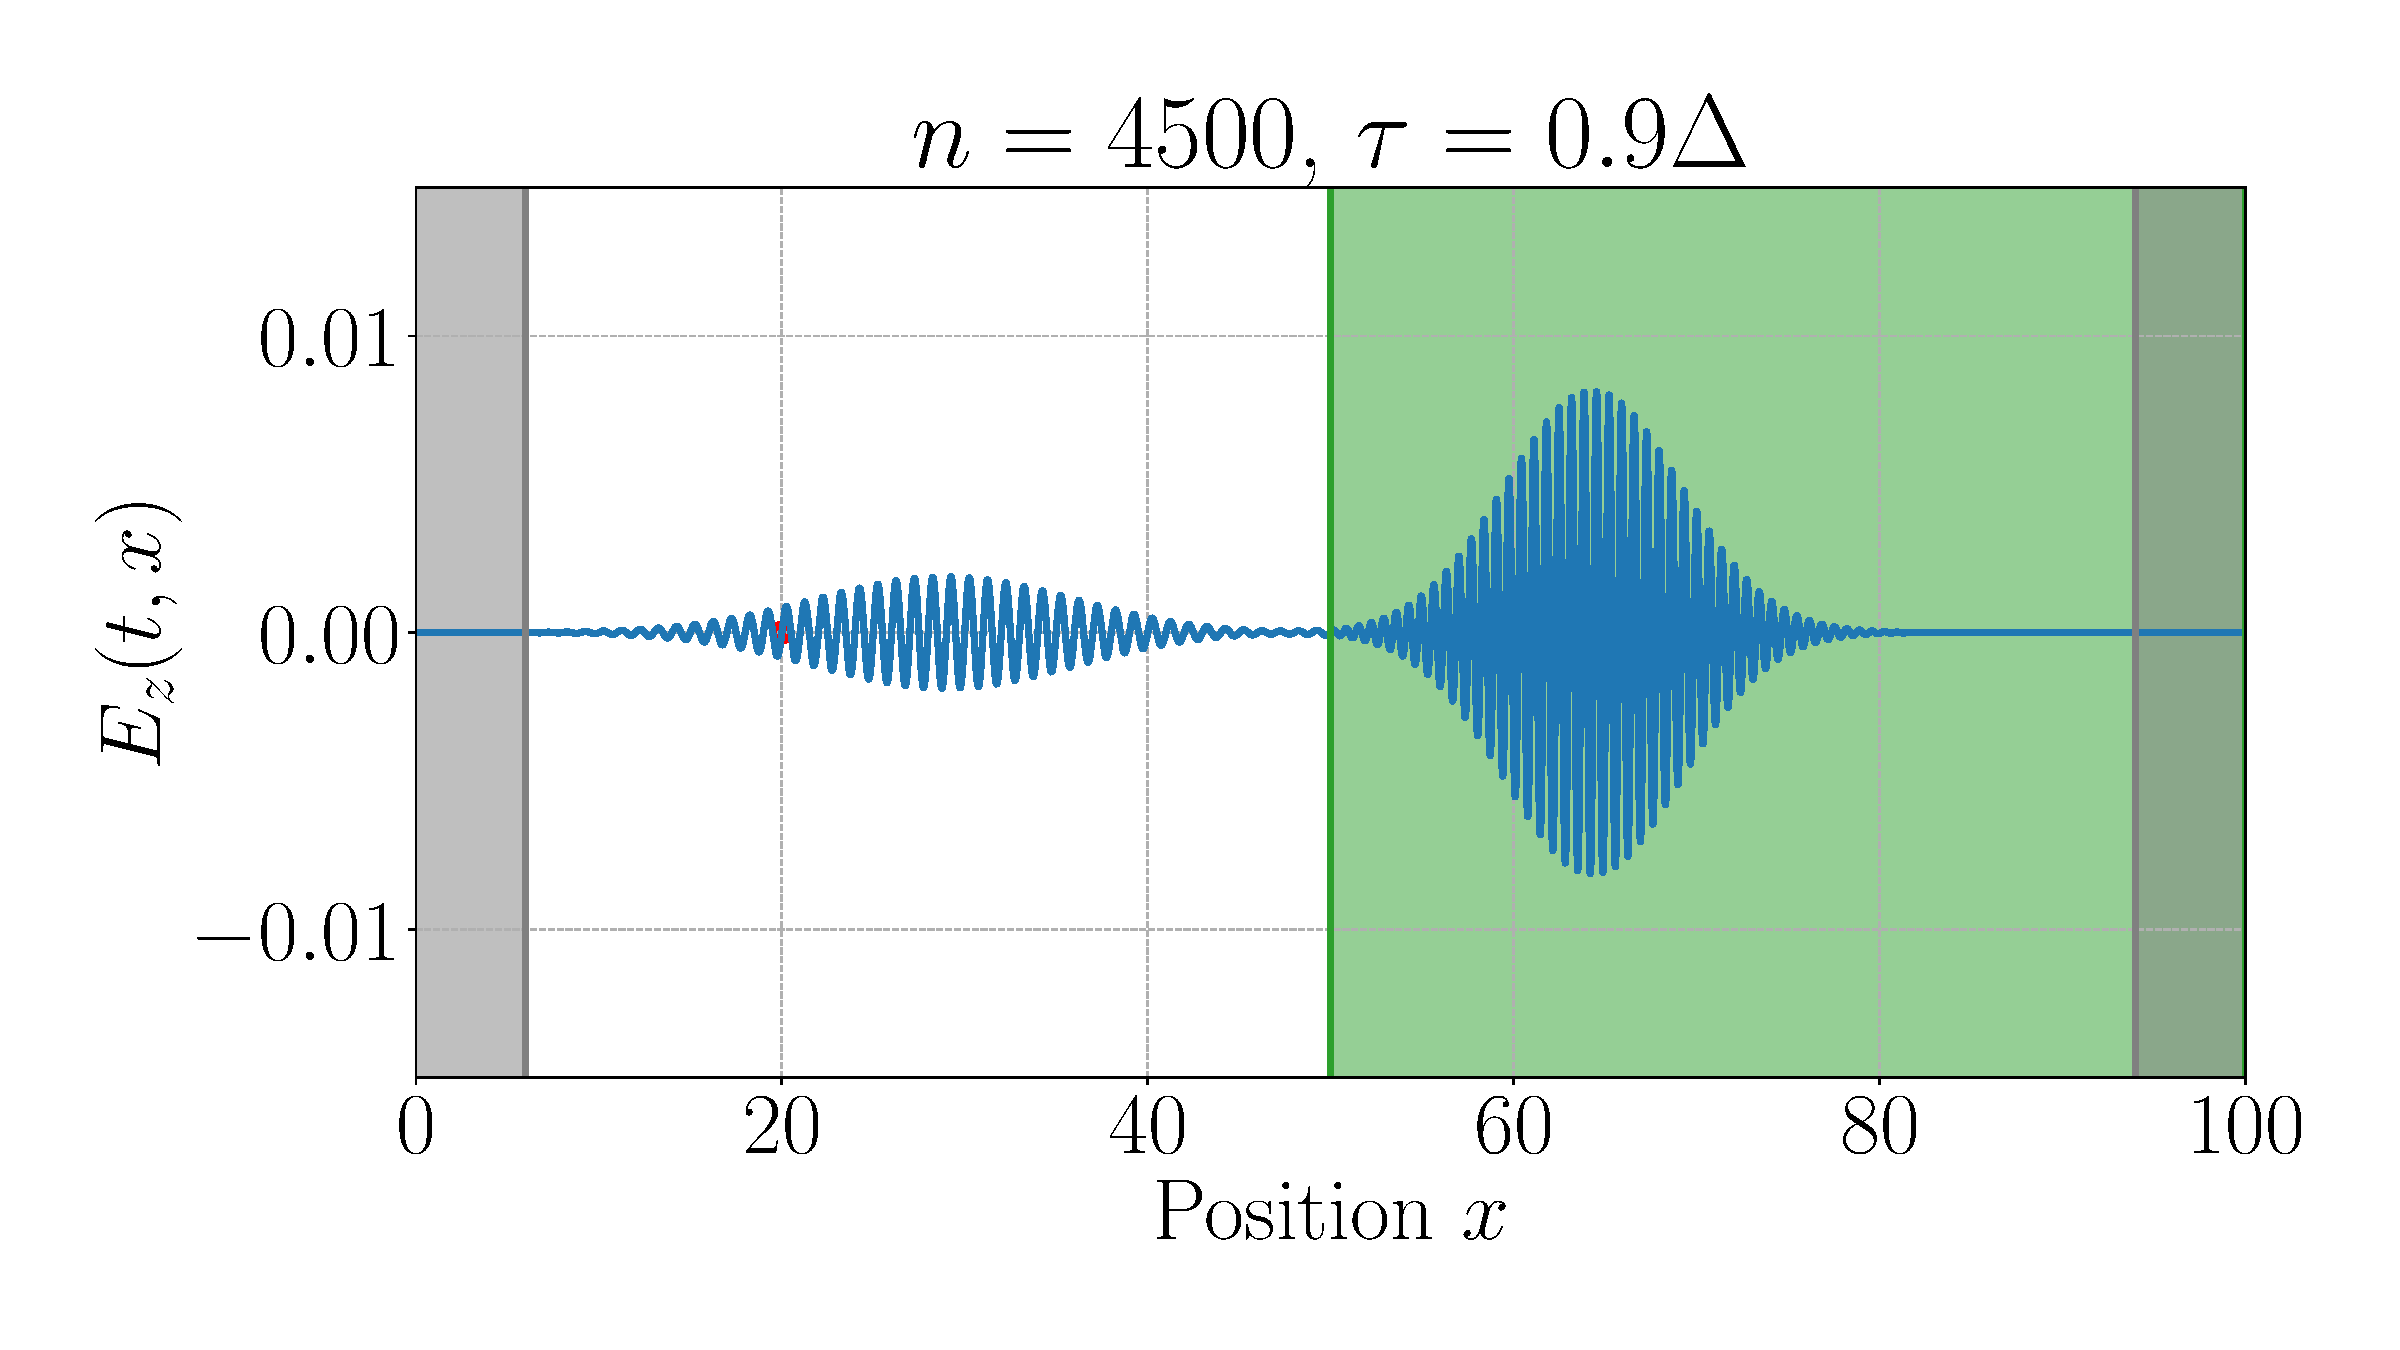
\includegraphics[width=\textwidth]{Plots/maxwell_tau0.9_thickglass_nmax4500.pdf}
         \caption{}
         \label{fig: thick_t80_tau09}
     \end{subfigure}
     \begin{subfigure}[h]{0.499\textwidth}
         \centering
         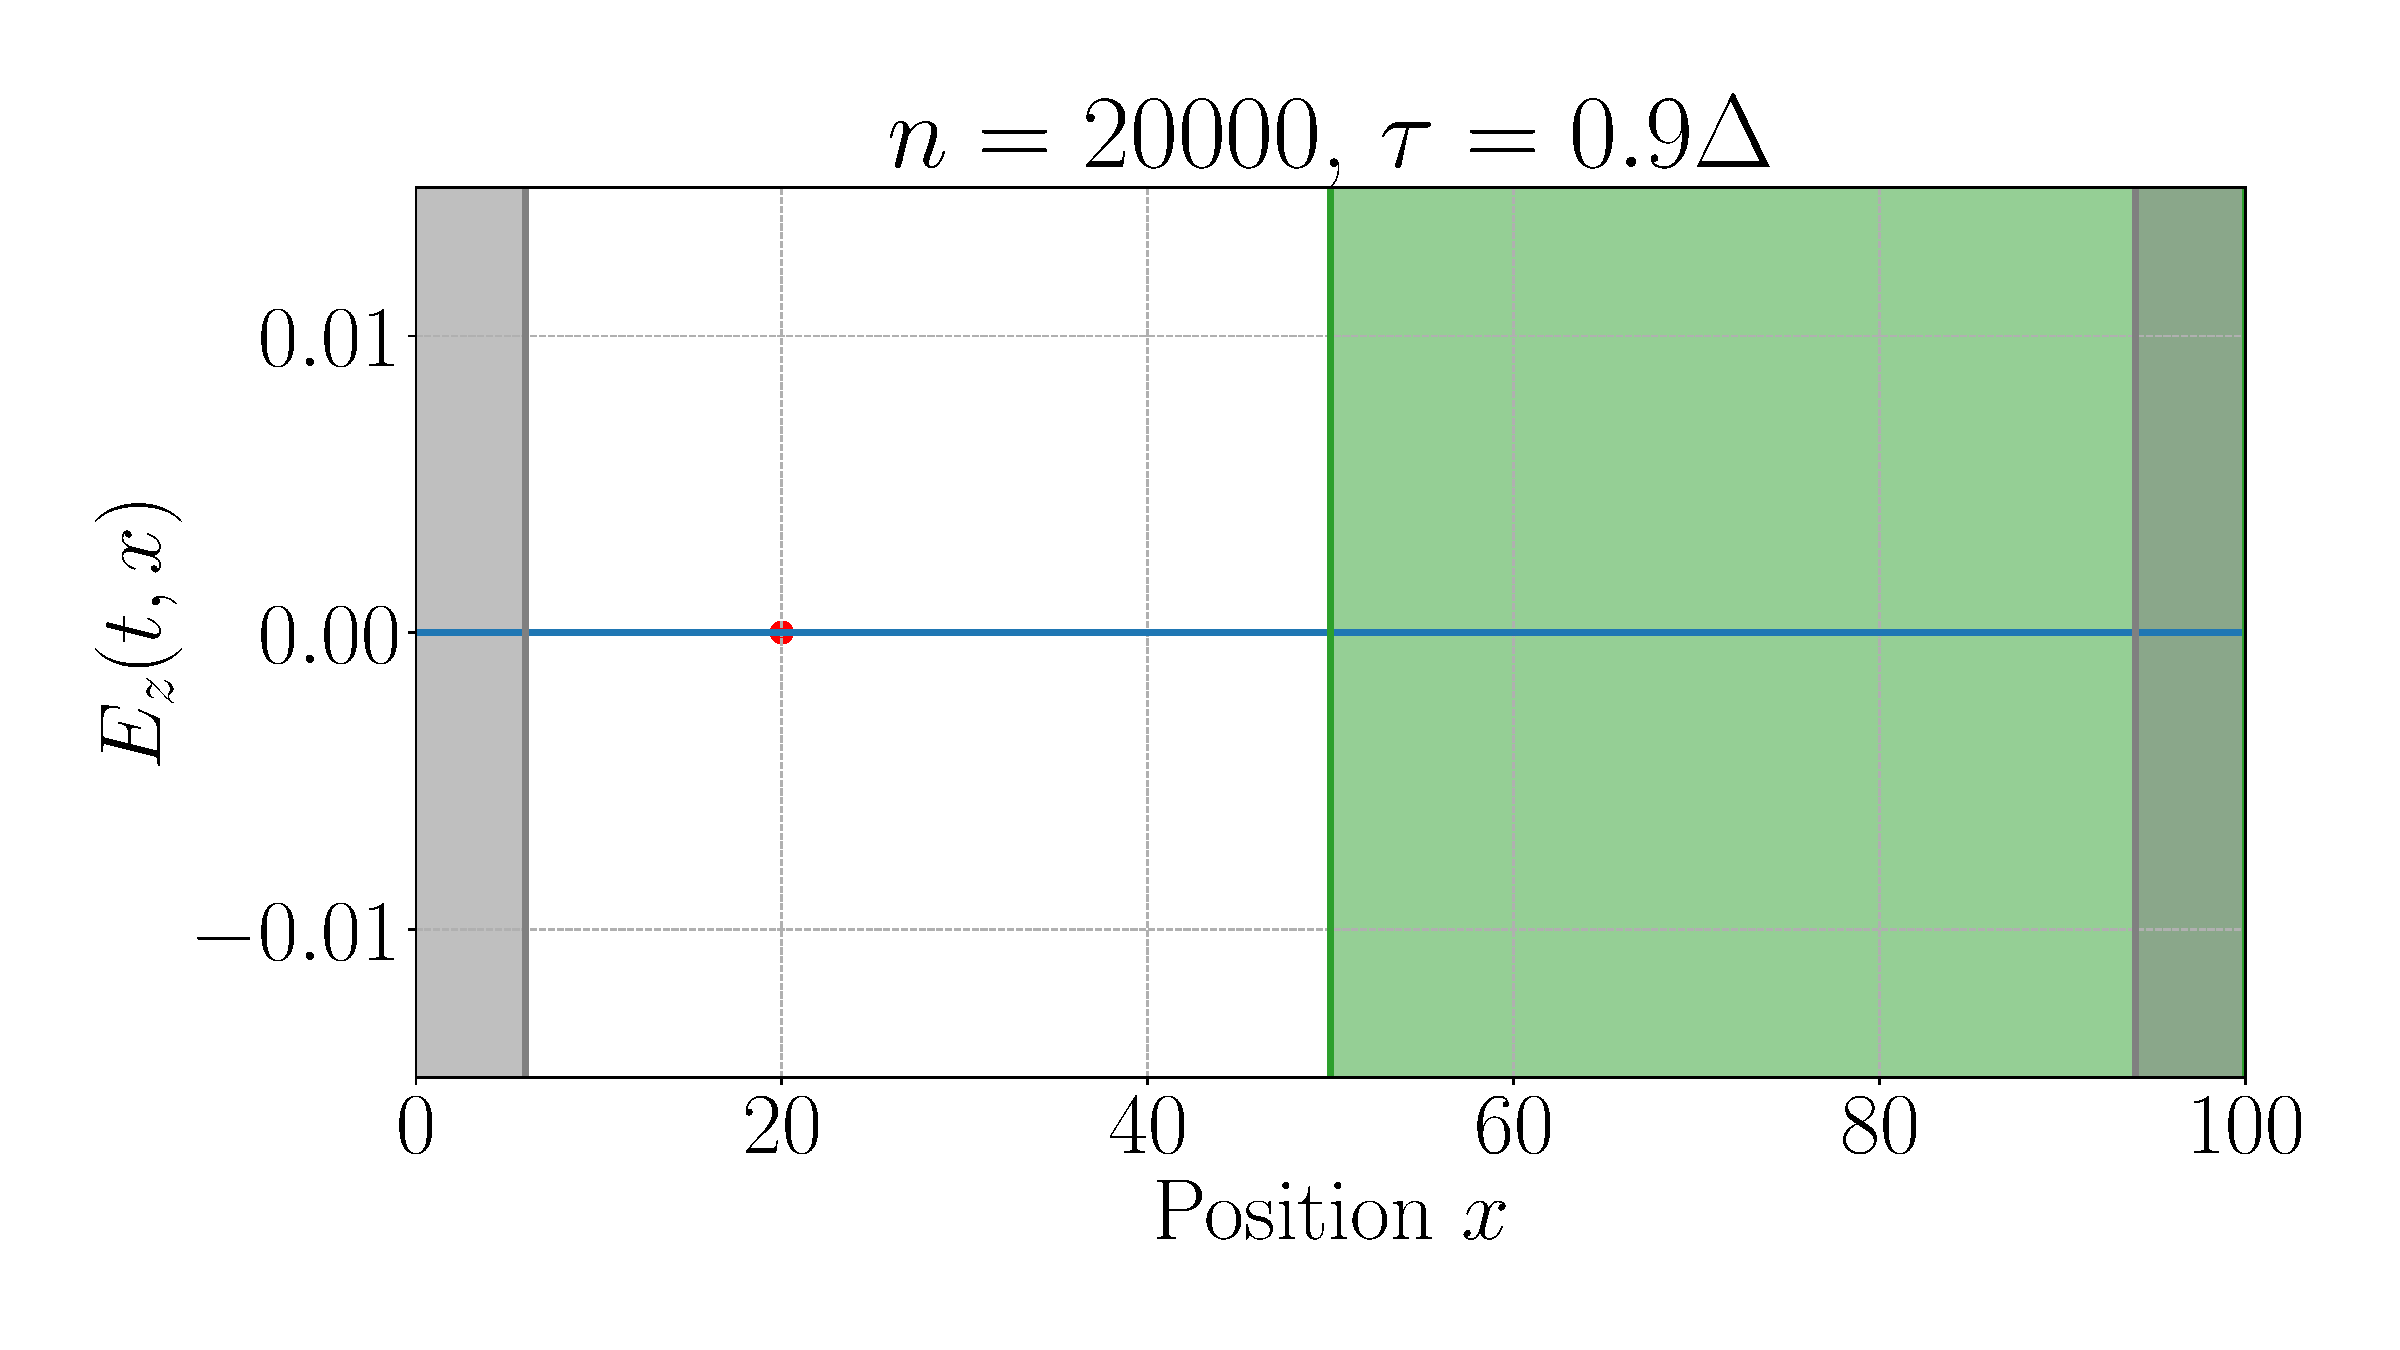
\includegraphics[width=\textwidth]{Plots/maxwell_tau0.9_thickglass_nmax20000.pdf}
         \caption{}
         \label{fig: thick_t500_tau09}
     \end{subfigure}
     \begin{subfigure}[h]{0.499\textwidth}
         \centering
         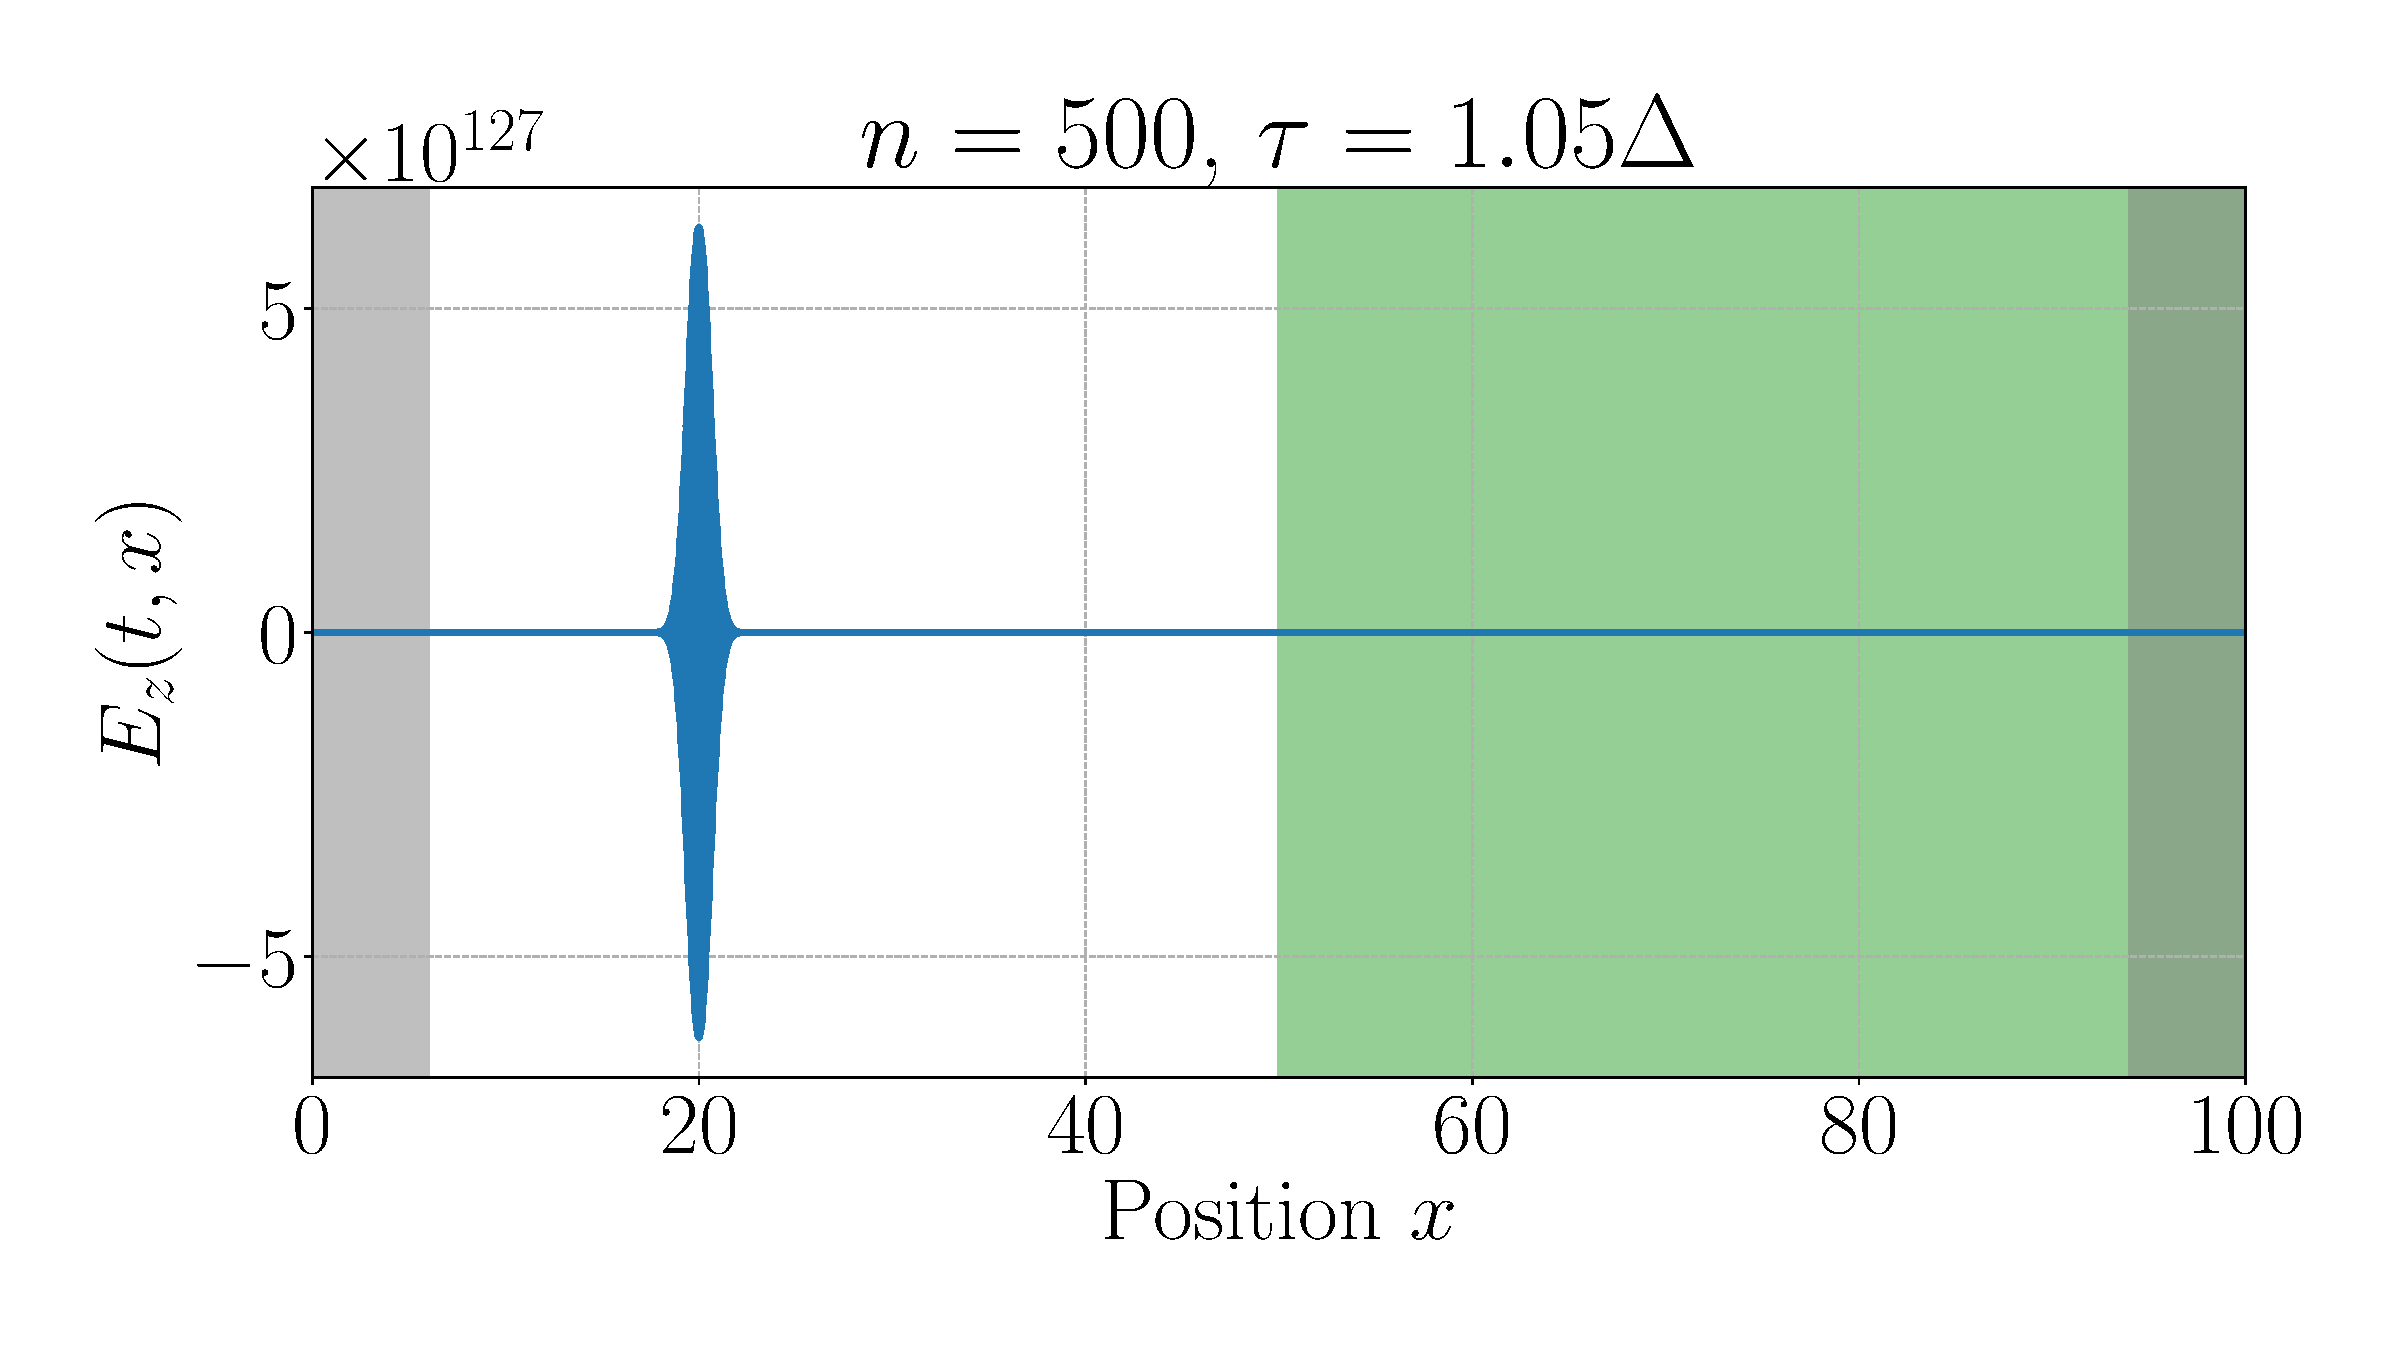
\includegraphics[width=\textwidth]{Plots/maxwell_tau1.05_thickglass_nmax500.pdf}
         \caption{}
         \label{fig: thick_t10_tau105}
     \end{subfigure}
\caption{Numerical solutions of the Maxwell equations using the Yee algorithm in one dimension for the system with the thick glass plate. The figures show the z-component of the electric field. The plots contain the glass plate in green and the insulator insulators in grey. The discretizations are $\lambda=1$, $\Delta=\lambda/50=0.02$, $X=L\Delta=100 \lambda=100$, and $L=5000$. The plots show the solution of the algorithm at different times and time discretizations: (a) $n=0$ $(t\approx 0)$ (b) $n=2500$ $(t\approx 45)$, (c) $n=3500$ $(t\approx 63)$, (d) $n=4500$ $(t\approx 81)$, and (e) $n=20000$ $(t\approx360)$, and $\tau=1.05 \Delta=0.021$ for (f) $n=500$ $(t\approx 9)$.}
\label{fig: Maxwell_thick}
\end{figure}

Furthermore, according to \refEq{eq: R} and the described method, we determined the following result for the reflection coefficient $R$

\begin{equation}
    R = 0.03537
    %0.034965959415691715
\end{equation}

\clearpage
\section{Discussion}
First, in \refFig{fig: Maxwell_thin}, we present the results for the system with a thin glass plate at five different times, with the initial value $n=0$ in \refFig{fig: sketch}. We first discuss the results for $\tau = 0.9 \Delta$ in figs. ((a)-(e)), followed by the results for $\tau = 1.05 \Delta$ in fig. (f). In \refFig{fig: thin_t40_tau09}, we observe that the source at $x_s$ generates two wavepackets in opposite directions. The left-moving wave is mostly absorbed by the insulator (grey regions), while the right-moving wave passes through the glass plate. In \refFig{fig: thin_t60_tau09}, we observe that the amplitude inside the glass is smaller, which results from interference with reflected waves. In \refFig{fig: thin_n3505_tau09}, we see that at $n=3510$, the amplitude inside the glass matches outside, confirming the previous observation. At $n=4500$, three wavepackets are visible: one transmitted wave and two reflected waves from the glass sides. At $n=20000$, all waves are absorbed at the boundaries. These results match our physical expectations, validating the choice of $\tau = 0.9 \Delta$.

For $\tau = 1.05 \Delta$, shown in \refFig{fig: thin_t10_tau105}, the amplitude diverges, indicating numerical instability when the Courant condition is violated, as seen with an amplitude of $10^{127}$ at $n=500$.

Next, we present results for the system with a thick glass plate in \refFig{fig: Maxwell_thick}. The behavior at $\tau = 0.9 \Delta$ is similar to the thin glass case. At $n=3500$, the wave transmitted into the glass has a smaller amplitude, while interference causes a larger amplitude outside the glass. The reflected and transmitted waves are clearer in \refFig{fig: thick_t80_tau09} at $n=4500$, and all waves are absorbed at $n=20000$.

For $\tau = 1.05 \Delta$, the results are similar to the thin glass case, with an amplitude of order $10^{127}$, confirming numerical instability.

Finally, the reflection coefficient $R$ was calculated and compared to the theoretical value. We find:
\[
    |R_{theory} - R| = 4 \cdot 10^{-4}.
\]
This small difference, within numerical uncertainties, confirms the accuracy of our simulation, and we conclude that the Yee-algorithm provides reasonable physical results.
\clearpage


\end{document}